
\scsection{Введение в описание внутреннего языка ostis-систем (компьютерных систем, построенных по Технологии OSTIS) и близких ему внешних языков, используемых для представления исходных текстов баз знаний}
\label{intro_lang}

\begin{SCn}

\scnsectionheader{\currentname}
\scnreltovector{конкатенация}{\nameref{intro_sc_code};\nameref{intro_scg};\nameref{intro_scs};\nameref{intro_scn}}

\scntext{семантическое включение}{Поскольку текст данной публикации представляет собой исходный текст основной части базы знаний соответствующий ostis-системы, необходимо сразу во вводном разделе публикации пояснить некоторые принципы, лежащие в основе представления баз знаний в памяти ostis-систем, а также некоторые правила и условные обозначения, используемые в оформлении исходных текстов баз знаний ostis-систем. 

Подчеркнем, что все эти принципы, правила и условные обозначения детально рассмотрены в соответствующих разделах, но некоторые из них необходимо пояснить до начала ознакомления с основными положениями Технологии OSTIS. Фактически речь идет о кратком руководстве конечных пользователей ostis-систем. 

Для представления баз знаний ostis-систем используется целый ряд как универсальных языков, так и специализированных языков, как формальных языков, так и неформальных языков, как внутренних языков, обеспечивающих представление информации в памяти ostis-систем, так и внешних языков, обеспечивающих представление информации, вводимой в память ostis-систем, либо выводимой из этой памяти. Неформальные языки используются исключительно для представления файлов, хранимых в памяти ostis-системы и формально специфицируемых в рамках базы знаний этой ostis-системы. 

На множестве языков, используемых ostis-системами, задаётся целый ряд отношений. Язык $\bm{L_i}$ и язык $\bm{L_j}$ будем считать \textit{семантически эквивалентными языками*} в том и только в том случае, если для каждого текста, принадлежащего языку $\bm{L_i}$, существует \textit{семантически эквивалентный текст*}, принадлежащий языку $\bm{L_j}$, и наоборот. 

Язык $\bm{L_j}$ будем считать \textit{семантическим расширением*} языка $\bm{L_i}$ в том и только в том случае, есть ли для каждого текста, принадлежащего языку $\bm{L_i}$, существует \textit{семантически эквивалентный текст*}, принадлежащий языку $\bm{L_j}$, но обратное неверно. 

Язык $\bm{L_j}$ будем считать \textit{синтаксическим расширением*} языка $\bm{L_i}$ в том и только в том случае, если:

\begin{scnitemize}
\item $\bm{L_j} \supset \bm{L_i}$ (то есть все тексты языка $\bm{L_i}$ являются также и текстами языка $\bm{L_j}$, но обратное неверно);
\item Язык $\bm{L_j}$ и язык $\bm{L_i}$ являются \textit{семантически эквивалентными языками*}.
\end{scnitemize}

В основе ostis-систем лежат четыре универсальных и, следовательно, \textit{семантически эквивалентных языка*}: 
\begin{scnitemize}
\item SC-код (Semantic Computer Code) -- \textit{внутренний язык*} ostis-систем; 
\item SCg-код (Semantic Code graphical) -- \textit{внешний язык*} ostis-систем, тексты которого представляют собой графовые структуры общего вида с точно \textit{денотационной семантикой};
\item SCs-код (Semantic Code string) -- внешний язык ostis-систем, который предназначен для обмена сообщениями между ostis-системами и тексты которого представляют собой строки (цепочки) символов;
\item SCn-код (Semantic Code natural) -- внешний язык ostis-систем, который предназначен для оформления \textit{исходных текстов баз знаний} ostis-систем и тексты которого представляют собой двухмерные матрицы символов, являющиеся результатом форматирования, двухмерной структуризации текстов SCs-кода.
\end{scnitemize}

Для эксплуатации интеллектуальных компьютерных систем,  построенных на основе \textit{SC-кода}, кроме способа абстрактного внутреннего представления баз знаний (SC-кода) потребуются несколько способов внешнего изображения абстрактных \textit{sc-конструкций}, удобных для пользователей и используемых при оформлении исходных текстов баз знаний указанных интеллектуальных компьютерных систем и исходных текстов фрагментов этих баз знаний, а также используемых для отображения пользователям различных фрагментов баз знаний по пользовательским запросам. В качестве таких способов внешнего изображения \textit{sc-конструкций} предлагается \textit{SCg-код} и \textit{SCn-код}.

Для описания перечисленных языков, используемых ostis-системами, в каждом из них мы выделим \textit{ядро языка*}, которое является \textit{семантически эквивалентным языком*} для соответствующего языка и имеет минимальную синтаксическую сложность. Описание каждого из указанных языков строится как описание семейства языков, являющихся различного вида \textit{синтаксическими расширениями*} соответствующего языка-ядра.
}

\end{SCn}


\scsubsection{Введение в описание внутреннего языка ostis-систем}
\label{intro_sc_code}

\begin{SCn}

\scnsectionheader{\currentname}

\scnstartsubstruct

\scnsegmentheader{Основные положения внутреннего языка ostis-систем}
\scnstartsubstruct

\scnheader{\currentname}
\scnreltovector{конкатенация сегментов}{Основные положения внутреннего языка ostis-систем;Описание Ядра SC-кода;SC-код как синтаксическое расширение Ядра SC-кода;Использование SC-кода для формального описания собственного синтаксиса}

\scnheader{SC-код}
\scnidtf{Язык унифицированного смыслового представления знаний в памяти интеллектуальных компьютерных систем}
\scnidtf{Внутренний язык ostis-систем}
\scnrelto{внутренний язык}{ostis-система}
\scntext{эпиграф}{Информация содержится не в самих знаках, а в конфигурации связей между ними.}
\scntext{эпиграф}{Он вскочил на коня и поскакал во все стороны.}

\scntext{основной внешний идентификатор sc-элемента}{SC-код}
\scnaddlevel{1}
\scniselement{имя собственное}
\scnaddlevel{-1}
\scntext{часто используемый неосновной внешний идентификатор sc-элемента}{sc-текст}
\scnaddlevel{1}
\scniselement{имя нарицательное}
\scnaddlevel{-1}
\scniselement{абстрактный язык}
\scnaddlevel{1}
    \scnidtf{Язык, для которого не уточняется способ представления символов (синтаксически элементарных фрагментов), входящих в состав текстов этого языка, а задается только \uline{алфавит*} этих символов, то есть семейство классов символов, считающихся синтаксически эквивалентными друг другу.}
    \scnaddlevel{1}
        \scnnote{Каждому абстрактному языку можно поставить в соответствие целое семейство \textit{реальных языков}, обеспечивающих \uline{изоморфное} реальное представление текстов указанного абстрактного языка путем уточнения способов представления (изображения, кодирования) символов, входящих в состав этих текстов, а также путем уточнения правил установления синтаксической эквивалентности этих символов. Очевидно, что во всём остальном синтаксис и денотационная семантика указанных реальных языков полностью совпадает с синтаксисом и денотационной семантикой соответствующего абстрактного языка.}
        \scnaddlevel{1}
            \scnnote{Для SC-кода как абстрактного языка необходима разработка как минимум трех синтаксически и семантически эквивалентных ему реальных языков: (1) язык кодирования текстов SC-кода в памяти традиционных компьютеров; (2) язык кодирования текстов SC-кода в семантической ассоциативной памяти; (3) Ядро SCg-кода -- язык, синтаксически и семантически эквивалентный SC-коду и обеспечивающий графическое представление текстов SC-кода.}
        \scnaddlevel{-1}
    \scnaddlevel{-1}
\scnaddlevel{-1}
\scniselement{графовый язык}
\scnaddlevel{1}
    \scnexplanation{язык, каждый текст которого (1) задается множеством входящих в него элементарных фрагментов (символов), которое, в свою очередь, состоит из (1.1) из множества узлов (вершин), возможно, синтаксически разного вида и (1.2) из множества связок, которые также могут принадлежать разным синтаксически выделяемым классам, а также (2) задается в общем случае несколькими отношениями инцидентности связок с компонентами этих связок (при этом указанными компонентами в общем случае могут быть не только вершины, но и другие связки).}
\scnaddlevel{-1}

\scnidtf{Универсальный язык, обеспечивающий внутреннее представление и структуризацию \uline{всех}(!), используемых ostis-системой в процессе своего функционирования.}
\scnidtf{Универсальный язык, являющийся результатом унификации (уточнения) синтаксиса и денотационной семантики семантических сетей.}
\scnaddlevel{1}
    \scnexplanation{Универсальность SC-кода обеспечивается и тем, что элементами текстов SC-кода могут быть знаки описываемых сущностей \uline{любого} вида, в том числе, и  знаки связей между описываемыми сущностями и/или их знаками}
    \scnaddlevel{1}
        \scntext{следствие}{Тексты SC-кода являются графовыми структурами расширенного вида, в которых знаки описываемых связей могут соединять не только вершины (узлы) графовой структуры, но и знаки других связей.}
    \scnaddlevel{-1}
\scnaddlevel{-1}
\scnidtf{Базовый универсальный язык внутреннего представления знаний в памяти ostis-систем.}
\scnidtf{Базовый внутренний язык ostis-систем.}
\scnidtf{Максимальный внутренний язык ostis-систем, по отношению к которому все остальные (специализированные) внутренние языки являются его подъязыками (подмножествами)}
\scnidtf{Множество всевозможных текстов SC-кода}
\scnaddlevel{1}
\scniselement{имя собственное}
\scnaddlevel{-1}
\scnidtf{текст SC-кода}
\scnaddlevel{1}
\scniselement{имя нарицательное}
\scnaddlevel{-1}


\filemodetrue
\scnrelfromvector{принципы, лежащие в основе}{\textit{Знаки} (обозначения) всех \textit{сущностей}, описываемых в \textit{sc-текстах} (текстах \textit{\textbf{SC-кода}}) представляются в виде синтаксически элементарных (атомарных) фрагментов \textit{sc-текстов} и, следовательно, не имеющих внутренней структуры, не состоящих из более простых фрагментов \textit{текста}, как, например, имена (термины), которые представляют \textit{знаки} описываемых \textit{сущностей} в привычных \textit{языках} и состоят из \textit{букв}.;\textit{Имена} (термины), \textit{естественно-языковые тексты} и другие информационные конструкции, не являющиеся \textit{sc-текстами}, могут входить в состав \textit{sc-текста}, но только как \textit{файлы}, описываемые (специфицируемые) \textit{sc-текстами}. Таким образом, в состав базы знаний \textit{интеллектуальной компьютерной системы}, построенной на основе \textit{\textbf{SC-кода}}, могут входить \textit{имена} (термины), обозначающие некоторые описываемые \textit{сущности} и представленные соответствующими \textit{файлами}. Каждый \textit{sc-элемент} будем называть внутренним обозначением некоторой \textit{сущности}, а \textit{имя} этой \textit{сущности}, представленное соответствующим файлом, будем называть \textit{внешним идентификатором} (внешним обозначением) этой \textit{сущности}. При этом каждый именуемый (идентифицируемый) \textit{sc-элемент} связывается дугой, принадлежащей отношению ``быть \textit{\textbf{внешним идентификатором*}}~'', с \textit{узлом}, содержимым которого является \textit{файл} идентификатора (в частности, \textit{имени}), обозначающего ту же \textit{сущность}, что и указанный выше \textit{sc-элемент}. \textit{Внешним идентификатором} может быть не только \textit{имя} (термин), но и иероглиф, пиктограмма, озвученное имя, жест. Особо отметим, что \textit{внешние идентификаторы} описываемых \textit{сущностей} в \textit{интеллектуальной компьютерной системе}, построенной на основе \textit{\textbf{SC-кода}}, используются только (1) для анализа информации, поступающей в эту систему из вне из различных источников, и ввода (понимания и погружения) этой информации в \textit{базу знаний}, а также (2) для синтеза различных \textit{сообщений}, адресуемых различным субъектам (в т.ч. пользователям).;Тексты \textit{\textbf{SC-кода}} (\textit{sc-тексты}) имеют в общем случае нелинейную (графовую) структуру, поскольку (1) \textit{знак} каждой описываемой сущности входит в состав \textit{sc-текста} однократно и (2) каждый такой \textit{знак} может быть инцидентен неограниченному числу других \textit{знаков}, поскольку каждая описываемая \textit{сущность} может быть связана неограниченным числом связей с другими описываемыми \textit{сущностями}.;
\textit{База знаний}, представленная текстом \textit{\textbf{SC-кода}}, является \textit{графовой структурой} специального вида, алфавит элементов которой включает в себя множество \textit{узлов}, множество \textit{ребер}, множество \textit{дуг}, множество \textit{базовых дуг} -- дуг специально выделенного типа, обеспечивающих структуризацию \textit{баз знаний}, а также множество специальных \textit{узлов}, каждый из которых имеет содержимое, являющееся \textit{файлом}, хранящимся в памяти \textit{интеллектуальной компьютерной системы}. Структурная особенность данной \textit{графовой структуры} заключается в том, что ее \textit{дуги} и \textit{ребра} могут связывать не только \textit{узел} с \textit{узлом}, но и \textit{узел} с \textit{ребром} или \textit{дугой}, \textit{ребро} или \textit{дугу} с другим \textit{ребром} или \textit{дугой}.;
\uline{Все элементы} (\textit{sc-элементы}) указанной выше \textit{графовой структуры} (текста \textit{\textbf{SC-кода}}), т.е. все ее узлы (sc-узлы), ребра (sc-ребра) и дуги (sc-дуги) являются обозначениями различных сущностей. При этом ребро является обозначением бинарной неориентированной связки между двумя сущностями, каждая из которых либо представлена в рассматриваемой графовой структуре соответствующим знаком, либо является самим этим знаком. Дуга является обозначением бинарной ориентированной связки между двумя сущностями. Дуга специального вида (\textit{\textbf{базовая дуга}}) является знаком связи между узлом, обозначающим некоторое множество элементов рассматриваемой графовой структуры, и одним из элементов этой графовой структуры, который принадлежит указанному множеству. Узел, имеющий содержимое (узел, для которого содержимое существует, но может в текущий момент быть неизвестным) является знаком файла, который является содержимым этого узла. Узел, не являющийся знаком файла, может обозначать какой-либо материальный объект, первичный абстрактный объект(например, число, точку в некотором абстрактном пространстве), какую-либо бинарную связь, какое-либо множество (в частности, понятие, структуру, ситуацию, событие, процесс). При этом сущности, обозначаемые элементами рассматриваемой графовой структуры, могут быть постоянными (существующими всегда) и временными (сущностями, которым соответствует отрезок времени их существования). Кроме того, сущности, обозначаемые элементами рассматриваемой графовой структуры, могут быть константными (конкретными) сущностями и переменными (произвольными) сущностями. Каждому элементу рассматриваемой графовой структуры, являющемуся обозначением переменной сущности, ставится в соответствие область возможных значений этого обозначения. Область возможных значений каждого переменного ребра является подмножеством множества всевозможных константных ребер, область возможных значений каждой переменной дуги является подмножеством множества всевозможных константных дуг, область возможных значений каждого переменного узла является подмножеством множества всевозможных константных узлов.;
В рассматриваемой графовой структуре, являющейся представлением базы знаний в \textit{\textbf{SC-коде}}, могут, но не должны существовать разные элементы графовой структуры, обозначающие одну и ту же сущность. Если пара таких элементов обнаруживается, то эти элементы склеиваются (отождествляются). Таким образом, синонимия внутренних обозначений в базе знаний интеллектуальной компьютерной системы, построенной на основе \textit{\textbf{SC-кода}}, запрещена. При этом синонимия внешних обозначений считается нормальным явлением. Формально это означает, что из некоторых элементов рассматриваемой графовой структуры выходит несколько дуг, принадлежащих отношению ``быть \textit{\textbf{внешним идентификатором*}}~''. Из всех указанных дуг, принадлежащих отношению ``быть \textit{\textbf{внешним идентификатором*}}~'' и выходящих из одного элемента рассматриваемой графовой структуры, обязательно выделяется одна (очень редко две) путем включения их в число дуг, принадлежащих отношению ``быть \textit{\textbf{основным внешним идентификатором*}}~''. Это означает, что указываемый таким образом внешний идентификатор не является омонимичным, т.е. не может быть использован как внешний идентификатор, соответствующий другому элементу рассматриваемой графовой структуры.;
Кроме файлов, представляющих различные внешние обозначения (имена, иероглифы, пиктограммы), в памяти интеллектуальной компьютерной системе, построенной на основе \textit{\textbf{SC-кода}}, могут хранится файлы различных текстов (книг, статей, документов, примечаний, комментариев, пояснений, чертежей, рисунков, схем, фотографий, видео-материалов, аудио-материалов).;
\uline{Любую сущность}, требующую описания, в тексте \textit{\textbf{SC-кода}} можно обозначить в виде \textit{sc-элемента}. Это являетс яодним из факторов, обеспечивающих универсальность \textit{\textbf{SC-кода}}. Особо подчеркнем, что sc-элементы являются не просто обозначениями различных описываемых сущностей, а обозначениями, которые являются элементарными (атомарными) фрагментами знаковой конструкции, т.е. фрагментами, детализация структуры которых не требуется для "прочтения"{} и понимания этой знаковой конструкции.;
Текст \textit{\textbf{SC-кода}}, как и любая другая графовой структура, является абстрактным математическим объектом, не требующим детализации (уточнения) его кодирования в памяти компьютерной системы (например, в виде матрицы смежности, матрицы инцидентности, списковой структуры). Но такая детализация потребуется для технической реализации памяти, в которой хранятся и обрабатываются sc-тексты.;
Важнейшим дополнительным свойством \textit{\textbf{SC-кода}} является то,что он удобен не просто для внутреннего представления знаний в памяти интеллектуальной компьютерной системы, но также и для внутреннего представления информации в памяти компьютеров, специально предназначенных для интерпретации семантических моделей интеллектуальных компьютерных систем. Т.е., \textit{\textbf{SC-код}} определяет синтаксические, семантические и функциональные принципы организации памяти компьютеров нового поколения, ориентированных на реализацию интеллектуальных компьютерных систем, -- принципы организации графодинамической ассоциативной семантической памяти.;
\textit{\textbf{SC-код}} рассматривается нами как объединение трех его подъязыков, в число которых входит \textit{\textbf{Ядро SC-кода}}, подъязык \textit{\textbf{SC-кода}}, обеспечивающий представление текстов \textit{\textbf{SC-кода}} (\textit{sc-текстов}) в форме орграфов классического вида, являющихся подразбиениями текстов \textit{\textbf{Ядра SC-кода}} и, соответственно, использующих \uline{явное} представление пар инцидентности элементов sc-текстов (sc-элементов), синтаксическое \textit{\textbf{Расширение Ядра SC-кода}}, обеспечивающее представление в памяти ostis-системы информационных конструкций инородного для \textit{\textbf{SC-кода}} вида.
}
\filemodefalse 
\scnaddlevel{1}
\scninlinesourcecommentpar{Завершили Описание принципов, лежащих в основе SC-кода}
\scnaddlevel{-1}

\scnheader{SC-код}
\scnnote{Следует особо подчеркнуть, что  унификация и максимально возможное упрощение  \textbf{\textit{синтаксиса}} и \textbf{\textit{денотационной семантики}} внутреннего языка интеллектуальных компьютерных систем прежде всего необходимы потому, что подавляющий объем \textbf{\textit{знаний}}, хранимых в составе  базы знаний интеллектуальной компьютерной системы, представляют собой \textbf{\textit{метазнания}}, описывающие свойства других знаний. К \textit{метазнаниям}, в частности, следует отнести и различного вида логические высказывания и всевозможного вида программы, описания методов (навыков), обеспечивающих решение различных классов задач. Необходимо исключить зависимость формы представляемого знания от вида этого знания. Форма (структура) внутреннего представления знания любого вида должна зависеть \uline{только}(!) от смысла этого знания. Более того, конструктивное (формальное) развитие теории интеллектуальных компьютерных систем невозможно без уточнения (унификации, стандартизации) и обеспечения семантической совместимости различных видов знаний, хранимых в базе знаний интеллектуальной компьютерной  системы.  Очевидно, что многообразие форм представления семантически эквивалентных знаний делает разработку общей теории  интеллектуальных компьютерных систем практически невозможной.}

\scnheader{SC-пространство}
\scnnote{Понятие SC-пространства наряду с понятием SC-кода играет важнейшую роль для уточнения и формализации понятия смысла информационных конструкций, для унификации смыслового представления информации и для максимально возможного исключения субъективизма в трактовке понятия смысла. Смысл информационной конструкции в конечном счете определяется (1) конфигурацией смыслового представления этой конструкции и (2) и "местоположением" (контекстом) смыслового представления указанной информационной конструкции в рамках смыслового пространства, т.е. в рамках объединенного смыслового представления \uline{всевозможных} информационных конструкций, либо в рамках объединенного смыслового представления информации, накопленной к заданному моменту времени некоторым индивидуальным субъектом или коллективом субъектов. Таким объединенным смысловым представлением информации, в частности, является смысловое представление глобальной базы всех знаний, накопленных человечеством к текущему моменту.}
\scnexplanation{Объединение (вместилище) \uline{всевозможных} унифицированных семантических сетей (текстов SC-кода)}
\scnaddlevel{1}
    \scnnote{При теоретико-множественном объединении текстов SC-кода семантически эквивалентные (синонимичные) элементы (синтаксически элементарные фрагменты) этих текстов считаются совпадающими элементами и при объединении указанных текстов "склеиваются".}
\scnaddlevel{-1}
\scnrelto{объединение}{SC-код}
\scnidtf{Унифицированное смысловое пространство}
\scntext{достоинство}{Важнейшим достоинством SC-пространства является возможность уточнения таких понятий, как понятие аналогичности (сходства и отличия) различных описываемых "внешних" сущностей, аналогичности унифицированных семантических сетей (текстов SC-кода), понятие семантической близости описываемых сущностей (в том числе, и текстов SC-кода).}

\scnendstruct \scninlinesourcecommentpar{Завершили сегмент ``Основные положения внутреннего языка ostis-систем''}

\scnsegmentheader{Описание Ядра SC-кода}
\scnstartsubstruct

\scnstructheader{Синтаксис Ядра SC-кода}
\scnstartsubstruct

\scnheader{Синтаксис Ядра SC-кода}
\scnnote{\textit{Синтаксис Ядра SC-кода} задается: (1) \textit{Алфавитом Ядра SC-кода}, (2) Отношением \textit{инцидентности sc-коннекторов*}, (3) Отношением \textit{инцидентности входящих sc-дуг*}}
\scnrelto{синтаксис}{Ядро SC-кода}

\scnheader{Ядро SC-кода}
\scnrelfrom{множество всех элементов конструкций данного языка}{sc-элемент}
\scnaddlevel{1}
    \scnidtf{элемент конструкции \textit{Ядра SC-кода}}
    \scnidtf{синтаксически элементарный (атомарный) фрагмент дискретной информационной конструкции, принадлежащей \textit{Ядру SC-кода}}
    \scnidtf{Класс элементов конструкций \textit{Ядра SC-кода}}
    \scnidtf{Множество всех элементов всевозможных конструкций \textit{Ядра SC-кода}}
\scnaddlevel{-1}
\scnrelfrom{алфавит}{Алфавит Ядра SC-кода\scnsupergroupsign}

\scnheader{Алфавит Ядра SC-кода\scnsupergroupsign}
\scnidtf{Множество (Семейство) всех классов синтаксически эквивалентных sc-элементов Ядра SC-кода}
\scnidtf{класс синтаксически эквивалентных sc-элементов Ядра SC-кода}
\scnidtf{класс синтаксически эквивалентных элементов конструкций Ядра SC-кода}
\scnidtf{элемент Алфавита Ядра SC-кода}
\scnidtf{синтаксический тип sc-элемента Ядра SC-кода}
\scnsubdividing{sc-узел общего вида;sc-ребро общего вида;sc-дуга общего вида;базовая sc-дуга}

\scnheader{sc-элемент}
\scnrelto{разбиение}{Алфавит Ядра SC-кода\scnsupergroupsign}
\scnaddlevel{1}
    \scnnote{\textit{Алфавит Ядра SC-кода} является одним из признаков классификации sc-элементов.}
    \scnnote{В процессе обработки текстов \textit{Ядра SC-кода} синтаксический тип \textit{sc-элементов} может меняться -- \textit{sc-узел} может трансформироваться в \textit{sc-ребро}, \textit{sc-ребро} -- в \textit{sc-дугу}, \textit{sc-дуга} общего вида -- в \textit{базовую sc-дугу}.}
\scnaddlevel{-1}

\scnheader{синтаксически выделяемый класс sc-элементов в рамках Ядра SC-кода\scnsupergroupsign}
\scnidtf{класс \textit{sc-элементов}, определяемый на основе \textit{Алфавита Ядра SC-кода}}
\scnhaselement{sc-коннектор}
\scnhaselement{sc-дуга}
\scnsuperset{Алфавит Ядра SC-кода\scnsupergroupsign}

\scnheader{sc-дуга}
\scnsubdividing{sc-дуга общего вида;базовая sc-дуга}

\scnheader{sc-коннектор}
\scnsubdividing{sc-ребро общего вида;sc-дуга общего вида}

\scnstructheader{Синтаксическая классификация sc-элементов в рамках Ядра SC-кода}
\scnstartstruct

\scnheaderlocal{sc-элемент}
\scnsubdividing{sc-узел общего вида;sc-коннектор\\
    \scnaddlevel{1}
    \scnsubdividing{sc-ребро общего вида;sc-дуга\\
    \scnaddlevel{1}
        \scnsubdividing{sc-дуга общего вида;базовая sc-дуга}
    \scnaddlevel{-1}
    }
    \scnaddlevel{-1}
    }
\bigskip
\scnendstruct

\scninlinesourcecommentpar{Завершили представление Синтаксической классификации sc-элементов в рамках Ядра SC-кода}
\scnnote{Все классы sc-элементов, входящие в состав синтаксической классификации sc-элементов являются синтаксически выделяемыми классами sc-элементов}

\scnheader{инцидентность sc-коннекторов*}
\scnidtfdef{Бинарное ориентированное отношение, первым компонентом каждой ориентированной пары которого является некоторый sc-коннектор, а вторым компонентом является один из sc-элементов, соединяемых указанным sc-коннектором с некоторым другим sc-элементом, который указывается в другой паре инцидентности для этого же sc-коннектора}

\scnheader{инцидентность входящих sc-дуг*}
\scnidtfdef{Бинарное ориентированное отношение, первым компонентом каждой ориентированной пары которого является некоторая sc-дуга, а вторым компонентом --- sc-элемент, в который указанная sc-дуга входит, т.е. sc-элемент, который является вторым компонентом, соединяемым (связываемым) указанной sc-дугой}

\scnheader{Ядро SC-кода}
\scnrelfrom{синтаксические правила}{\scnstructidtf{Синтаксические правила Ядра SC-кода}}
\scnaddlevel{1}
\scnhassubstruct{
\scnstartsetlocal\\
\scnaddlevel{1}
\scnheaderlocal{инцидентность sc-коннекторов*}\\
\scnsuperset{инцидентность входящих sc-дуг*}
\scniselement{бинарное ориентированное отношение}
\scnendstruct
\scnaddlevel{-1}
;\scnfileitem{Для каждого sc-коннектора существует две и только две пары \textit{инцидентности sc-коннекторов*}, указанный sc-коннектор является первым связующим компонентом. При этом для каждой sc-дуги из двух указанных пар инцидентности \uline{одна} должна принадлежать отношению инцидентности \textit{входящей sc-дуги*}.}
;\scnfileitem{Пары инцидентности sc-коннекторов могут быть \uline{кратными}. То есть sc-коннектор может соединять (связывать) sc-элемент с самим собой. Такие sc-коннекторы будем называть петлевыми sc-коннекторами (петлевыми sc-ребрами и петлевыми sc-дугами).}
;\scnfileitem{Само \textit{Отношение инцидентности sc-коннекторов*} и, следовательно, \textit{Отношение инцидентности входящих sc-дуг*} не имеет кратных пар инцидентности. То есть sc-коннектор не может быть инцидентен самому себе.}
;\scnfileitem{В область определения \textit{Отношения инцидентности sc-коннекторов*} и \textit{Отношения инцидентности входящих sc-дуг*} входят не только sc-узлы общего вида, но и sc-коннекторы. Это значит, что sc-коннектор может соединять (связывать) не только sc-узел с sc-узлом, но также sc-узел с sc-коннектором и даже sc-коннектор с sc-коннектором.}}
\scnaddlevel{1}
\scninlinesourcecommentpar{Завершили перечень синтаксических правил Ядра SC-кода}
\scnaddlevel{-2}
\bigskip
\scnendstruct \scninlinesourcecommentpar{Завершили изложение Синтаксиса Ядра SC-кода}

\scnstructheader{Денотационная семантика Ядра SC-кода}
\scnstartsubstruct

\scnheader{Ядро SC-кода}
\scnrelfrom{денотационная семантика}{Денотационная семантика Ядра SC-кода}
\scnaddlevel{1}
    \scnidtf{Описание соответствия информационных конструкций, принадлежащих \textit{Ядру SC-кода}, и сущностей, описываемых этими конструкциями}
\scnaddlevel{-1}

\scnheader{параметр, заданный на множестве sc-элементов}
\scnhaselement{Алфавит Ядра SC-кода\scnsupergroupsign}
\scnhaselement{Алфавит SC-кода\scnsupergroupsign}
\scnhaselement{Структурная типология sc-элементов\scnsupergroupsign}
\scnhaselement{Типология sc-элементов по признаку константности\scnsupergroupsign}
\scnhaselement{Типология sc-элементов по признаку постоянства обозначаемой сущности\scnsupergroupsign}
\scnhaselement{Типология sc-элементов по признаку доступности sc-элемента в процессе эксплуатации и эволюции базы знаний\scnsupergroupsign}

\scnstructheader{Семантическая классификация sc-элементов}
\scnstartsubstruct

\scnheader{sc-элемент}
\scnidtf{обозначение описываемой сущности}
\scnrelto{разбиение}{\scnkeyword{Структурная типология sc-элементов\scnsupergroupsign}}
\scnaddlevel{1} 
    \scneqtoset{обозначение терминальной сущности\\
    \scnaddlevel{1} 
    \scnsubdividing{обозначение материальной сущности\\
    \scnaddlevel{1} 
        \scnnote{К материальным сущностям относятся физические тела, поля, биологические объекты, технические системы и многое другое.}
    \scnaddlevel{-1}
    ;обозначение абстрактной терминальной сущности\\
    \scnaddlevel{1} 
        \scnnote{Примерами абстрактных терминальных сущностей являются предельно малые физические тела, точки различных пространств, числа.}
    \scnaddlevel{-1}
    ;обозначение дискретной информационной конструкции, не принадлежащей SC-коду\\
    \scnaddlevel{1} 
        \scnidtf{обозначение информационной конструкции, не являющейся конструкцией \textit{SC-кода} и тем более \textit{Ядра SC-кода}}
        \scnidtf{обозначение "инородной"{} для \textit{SC-кода} информационной конструкции}
        \scnsuperset{обозначение файла}
        \scnaddlevel{1}
            \scnidtf{обозначение внешней информационной конструкции, представленной в электронной форме}
        \scnaddlevel{-1}
    \scnaddlevel{-1}
    }
    \scnaddlevel{-1}
    ;обозначение sc-множества\\
    \scnaddlevel{1}
    \scnsubdividing{обозначение sc-связки;обозначение sc-класса;обозначение sc-структуры}
    \scnaddlevel{-1}
    }
\scnaddlevel{-1}

\scnheader{обозначение sc-связки}
\scnsubdividing{обозначение небинарной sc-связки;обозначение sc-пары\\
\scnaddlevel{1}
    \scnsubdividing{обозначение неориентированной sc-пары;обозначение ориентированной пары неизвестной направленности;обозначение ориентированной sc-пары\\
    \scnaddlevel{1}
        \scnsuperset{обозначение sc-пары принадлежности}
        \scnaddlevel{1}
            \scnsubdividing{обозначение позитивной sc-пары принадлежности;обозначение негативной sc-пары принадлежности;обозначение нечеткой sc-пары принадлежности}
        \scnaddlevel{-1}
    \scnaddlevel{-1}
    }
\scnaddlevel{-1}
}

\scnheader{sc-элемент}
\scnrelto{разбиение}{\scnkeyword{Типология sc-элементов по признаку константности\scnsupergroupsign}}
\scnaddlevel{1}
    \scneqtoset{sc-константа\\
    \scnaddlevel{1}
        \scnidtf{константный sc-элемент}
        \scnidtf{обозначение конкретной (фиксированной) сущности}
    \scnaddlevel{-1}
    ;sc-переменная\\
    \scnaddlevel{1}
        \scnidtf{переменный sc-элемент}
        \scnidtf{обозначение произвольной сущности из некоторого множества сущностей}
        \scnidtf{sc-элемент, имеющий (принимающий) произвольное значение из некоторого множества sc-элементов}
    \scnaddlevel{-1}
    }
\scnaddlevel{-1}
\scnrelto{разбиение}{\scnkeyword{Типология sc-элементов по постоянства обозначаемых сущностей\scnsupergroupsign}}
\scnaddlevel{1}
    \scneqtoset{обозначение постоянной сущности;обозначение временной сущности\\
    \scnaddlevel{1}
        \scnidtf{обозначение нестационарной сущности, факт существования которой зависит от времени}
        \scnsubdividing{обозначение прошлой сущности\\
        \scnaddlevel{1}
            \scnidtf{обозначение сущности, существовавшей до текущего момента времени}
        \scnaddlevel{-1}
        ;обозначение настоящей сущности\\
        \scnaddlevel{1}
            \scnidtf{обозначение сущности, существующей в текущий момент времени}
        \scnaddlevel{-1};обозначение будущей сущности\\
        \scnaddlevel{1}
            \scnidtf{обозначение сущности, существование которой прогнозируется или планируется в будущем}
        \scnaddlevel{-1}}
    \scnaddlevel{-1}
    }
\scnaddlevel{-1}
\scnrelto{разбиение}{\scnkeyword{Типология sc-элементов по признаку доступности sc-элемента в процессе эксплуатации и эволюции базы знаний\scnsupergroupsign}}
\scnaddlevel{1}
    \scneqtoset{удаленный sc-элемент\\
        \scnaddlevel{1}
            \scnidtf{sc-элемент, считающийся логически удаленным, но присутствующим в описании истории эксплуатации и эволюции базы знаний}
        \scnaddlevel{-1};настоящий sc-элемент\\
        \scnaddlevel{1}
            \scnidtf{sc-элемент, входящий в состав эксплуатируемой части базы знаний}
        \scnaddlevel{-1};будущий sc-элемент\\
        \scnaddlevel{1}
            \scnidtf{sc-элемент, планируемый для включения в состав эксплуатируемой части базы знаний}
        \scnaddlevel{-1}}
\scnaddlevel{-1}

\scnheader{обозначение sc-множества}
\scnidtf{обозначение множества sc-элементов}
\scnsubdividing{произвольное sc-множество\\
    \scnaddlevel{1}
        \scnidtf{sc-переменная, обозначающая произвольное sc-множество из некоторого семейства sc-множеств}
        \scnidtf{переменное sc-множество}
    \scnaddlevel{-1}
;sc-множество\\
    \scnaddlevel{1}
        \scnidtf{конкретное (константное, фиксированное) множество sc-элементов}
    \scnaddlevel{-1}}

\scnheader{sc-множество}
\scnidtf{множество sc-элементов}
\scnsubdividing{множество sc-констант\\
    \scnaddlevel{1}
        \scnidtf{множество, элементами которого являются только sc-константы}
    \scnaddlevel{-1}
    ;множество sc-переменных\\
    \scnaddlevel{1}
        \scnidtf{множество, элементами которого являются только sc-переменные}
        \scnsuperset{sc-переменная}
        \scnaddlevel{1}
            \scnidtf{множество, элементами которого являются всевозможные sc-переменные и только они}
            \scnsuperset{произвольное sc-множество}
            \scnaddlevel{1}
                \scnidtf{sc-переменная, значениями которой являются всевозможные обозначения sc-множеств и только они}
            \scnaddlevel{-1}
        \scnaddlevel{-1}
    \scnaddlevel{-1}
    ;множество sc-констант и sc-переменных\\
    \scnaddlevel{1}
        \scnidtf{sc-множество, в число элементов которого входят как sc-константы, так и sc-переменные}
        \scnsuperset{обозначение sc-множества}
            \scnaddlevel{1}
                \scnidtf{множество, элементами которого являются всевозможные sc-переменные и sc-константы, обозначающие sc-множества и только они}
            \scnaddlevel{-1}
    \scnaddlevel{-1}}

\scnheader{обозначение sc-связки}
\scnidtf{обозначение связи между sc-элементами и/или обозначаемыми ими сущностями}
\scnsubdividing{произвольная sc-связка\\
    \scnaddlevel{1}
        \scnidtf{sc-переменная, значениями которой являются обозначения sc-связок}
    \scnaddlevel{-1}
    ;sc-связка\\
    \scnaddlevel{1}
        \scnidtf{конкретная связка sc-элементов}
    \scnaddlevel{-1}
    }
\scnsuperset{обозначение sc-пары}
\scnaddlevel{1}
    \scnidtf{обозначение связки двух sc-элементов либо одного sc-элемента с самим собой}
    \scnsuperset{sc-пара}
    \scnaddlevel{1}
        \scnidtf{конкретная sc-пара}
        \scnsubset{sc-константа}
        \scnsuperset{sc-коннектор}
        \scnsuperset{ориентированная sc-пара}
        \scnaddlevel{1}
            \scnsuperset{sc-пара принадлежности}
            \scnaddlevel{1}
                \scnsubdividing{позитивная sc-пара принадлежности\\
                    \scnaddlevel{1}
                        \scnsuperset{позитивная постоянная sc-пара принадлежности}
                        \scnaddlevel{1}
                        \scnsuperset{базовая sc-дуга}
                        \scnaddlevel{-1}
                    \scnaddlevel{-1}
                ;негативная sc-пара принадлежности;нечеткая sc-пара принадлежности}
            \scnaddlevel{-1}
        \scnaddlevel{-1}
    \scnaddlevel{-1}
\scnaddlevel{-1}

\scnheader{обозначение sc-класса}
\scnidtf{обозначение множества sc-элементов, которые в соответствующем смысле эквивалентны друг другу, т.е. имеют одинаковые свойства}
\scnsubdividing{произвольный sc-класс\\
    \scnaddlevel{1}
        \scnsubset{sc-переменная}
        \scniselement{sc-константа}
    \scnaddlevel{-1}
    ;sc-класс\\
    \scnaddlevel{1}
        \scnsubset{sc-константа}
    \scnaddlevel{-1}
    }
    
\scnheader{sc-класс}
\scnsubdividing{sc-класс терминальных сущностей   ;sc-класс множеств\\
    \scnaddlevel{1}
        \scnsubdividing{sc-класс sc-связок\\
            \scnaddlevel{1}
                \scnsuperset{sc-отношение}
            \scnaddlevel{-1}
        ;sc-класс sc-классов\\
            \scnaddlevel{1}
                \scnsuperset{sc-параметр}
            \scnaddlevel{-1}
        ;sc-класс sc-структур\\
            \scnaddlevel{1}
                \scnsuperset{sc-язык}
                \scnaddlevel{1}
                    \scnidtf{специализированный язык, являющийся подъязыком SC-кода, и обеспечивающий представление всевозможных знаний в рамках соответствующей предметной области, которая, в свою очередь, специфицируется соответствующей комплексной онтологией}
                \scnaddlevel{-1}
            \scnaddlevel{-1}
        }
    \scnaddlevel{-1}
    }
\scnhaselement{обозначение sc-множества}
\scnaddlevel{1}
    \scnsuperset{sc-множество}
\scnaddlevel{-1}
\scnhaselement{sc-множество}
\scnhaselement{обозначение sc-связки}
\scnaddlevel{1}
    \scnsuperset{sc-связка}
\scnaddlevel{-1}
\scnhaselement{sc-связка}
\scnhaselement{обозначение sc-класса}
\scnaddlevel{1}
    \scnsuperset{sc-класс}
\scnaddlevel{-1}
\scnhaselement{sc-класс}
\scnhaselement{обозначение sc-структуры}
\scnaddlevel{1}
    \scnsuperset{sc-структура}
\scnaddlevel{-1}
\scnhaselement{sc-структура}
\scnhaselement{обозначение дискретной информационной конструкции}
\scnaddlevel{1}
    \scnsuperset{дискретная информационная конструкция}
    \scnaddlevel{1}
        \scnsuperset{файл}
        \scnaddlevel{1}
            \scnsuperset{файл ostis-системы}
            \scnaddlevel{1}
                \scnsuperset{внутренний файл ostis-системы}
            \scnaddlevel{-1}
        \scnaddlevel{-1}
    \scnaddlevel{-1}
    \scnsuperset{обозначение sc-структуры}
\scnaddlevel{-1}
\scnnote{Все семантически и синтаксически выделяемые классы sc-элементов, а также всевозможные подклассы этих классов являются экземплярами (элементами) \textit{sc-класса}}

\scnheader{обозначение sc-структуры}
\scnidtf{обозначение sc-множества, не являющегося ни sc-связкой, ни sc-классом}
\scnsubdividing{произвольная sc-структура\\
    \scnaddlevel{1}
        \scnsubset{sc-переменная}
    \scnaddlevel{-1}
;sc-структура\\
    \scnaddlevel{1}
        \scnidtf{конкретная sc-структура}
        \scnsubset{sc-константа}
    \scnaddlevel{-1}}

\scnendstruct \scninlinesourcecommentpar{Завершили представление \textit{Семантической классификации sc-элементов}}


\scnstructheader{Соотношение между семантически и синтаксически выделяемыми классами sc-элементов в рамках Ядра SC-кода}
\scnstartsubstruct

\scnheader{семантически выделяемый класс sc-элементов}
\scnidtf{класс sc-элементов, определяемый сущностями, которые обозначаются этими sc-элементами, также доступностью (активностью использования) sc-элементов в процессе эксплуатации и эволюции базы знаний}
\scniselement{обозначение терминальной сущности}
\scnaddlevel{1}
\scnsuperset{\scnkeyword{sc-узел общего вида}}
\scnaddlevel{-1}
\scniselement{обозначение небинарной sc-связки}
\scnaddlevel{1}
\scnsuperset{\scnkeyword{sc-узел общего вида}}
\scnaddlevel{-1}
\scniselement{обозначение sc-пары}
\scnaddlevel{1}
\scnrelboth{пара пересекающихся множеств}{sc-узел общего вида}
\scnsuperset{\scnkeyword{sc-коннектор}}
\scnnote{\textit{обозначение sc-пары} может быть представлено либо \textit{sc-узлом общего вида}, либо \textit{sc-коннектором}. При этом каждый \textit{sc-коннектор} представляет собой \textit{обозначение sc-пары}.}
\scnaddlevel{-1}
\scniselement{обозначение неориентированной sc-пары}
\scnaddlevel{1}
\scnidtf{обозначение бинарной неориентированной связи между sc-элементами}
\scnrelbothlist{пара пересекающихся множеств}{\scnkeyword{sc-узел общего вида};\scnkeyword{sc-ребро общего вида}}
\scnnote{\textit{обозначение неориентированной sc-пары} может быть представлено либо \textit{sc-узлом общего вида}, либо \textit{sc-ребром}. При этом не каждое \textit{sc-ребро} представляет обозначение \textit{неориентированный sc-пары}. Некоторые из них представляют \textit{обозначения ориентированных sc-пар неизвестной направленности}.}
\scnaddlevel{-1}
\scniselement{обозначение ориентированной sc-пары неизвестной направленности}
\scnaddlevel{1}
\scnrelbothlist{пара пересекающихся множеств}{\scnkeyword{sc-узел общего вида};\scnkeyword{sc-ребро общего вида}}
\scnaddlevel{-1}
\scniselement{обозначение ориентированной sc-пары}
\scnaddlevel{1}
\scnidtf{обозначение бинарной ориентированной связи между sc-элементами}
\scnrelbothlist{пара пересекающихся множеств}{\scnkeyword{sc-узел общего вида};\scnkeyword{sc-ребро общего вида}}
\scnsuperset{sc-дуга общего вида}
\scnaddlevel{-1}
\scniselement{константная постоянная позитивная sc-пара принадлежности}
\scnaddlevel{1}
\scnrelbothlist{пара пересекающихся множеств}{\scnkeyword{sc-узел общего вида};\scnkeyword{sc-ребро общего вида};\scnkeyword{sc-дуга общего вида}}
\scnsuperset{\scnkeyword{базовая sc-дуга}}
\scnreltoset{пересечение множеств}{sc-константа;обозначение постоянной сущности;обозначение sc-пары принадлежности}
\scnaddlevel{-1}
\scniselement{обозначение sc-класса}
\scnaddlevel{1}
\scnsubset{\scnkeyword{sc-узел общего вида}}
\scnaddlevel{-1}
\scniselement{обозначение sc-структуры}
\scnaddlevel{1}
\scnsubset{\scnkeyword{sc-узел общего вида}}
\scnaddlevel{-1}

\scnendstruct \scninlinesourcecommentpar{Завершили \textit{Описание Соотношения между семантически и синтаксически выделяемыми классами sc-элементов в рамках Ядра SC-кода}. В этом описании жирным курсивом выделены идентификаторы (имена) синтаксически выделяемых классов sc-элементов}

\scnheader{Ядро SC-кода}
\scnrelfrom{семантические правила}{\scnstructidtf{Семантические правила Ядра SC-кода}}
\scnaddlevel{1}
\scnhassubstruct{\scnfileitem{Каждый sc-элемент является знаком (обозначением) некоторой описываемой сущности.};\scnfileitem{Любая сущность может быть обозначена sc-элементом и, соответственно, описана в виде конструкции Ядра SC-кода.};\scnfileitem{С помощью sc-элементов можно описать любые связи между sc-элементами и/или между сущностями, которые обозначаются этими sc-элементами. При этом указанные связи трактуются как множества связываемых sc-элементов и обозначаются sc-ребрами, sc-дугами, а в случае небинарных связей -- sc-узлами.};\scnfileitem{Поскольку каждый sc-коннектор семантически трактуется как обозначение пары sc-элементов, связываемых (соединяемых) этим sc-коннектором, каждая пара инцидентности sc-коннектора семантически интерпретируется как обозначение пары принадлежности, связывающей sc-коннектор с одним из элементов обозначаемой им пары sc-элементов.};\scnfileitem{\uline{Любая} описываемая сущность может быть обозначена sc-узлом общего вида, но обратное неверно, т.к. некоторые сущности могут быть обозначены sc-ребрами общего вида, sc-дугами общего вида, базовыми sc-дугами.};\scnfileitem{Каждое sc-ребро является обозначением либо бинарной неориентированной связи между sc-элементами, либо бинарной ориентированной связи неизвестной направленности между sc-элементами.};\scnfileitem{Любая бинарная неориентированная связь между sc-элементами может быть обозначена sc-ребром, но обратное неверно.}}
\scnaddlevel{-1}
\bigskip

\scnendstruct \scninlinesourcecommentpar{Завершили описание Денотационной семантики Ядра SC-кода}

\scnheader{Правила синтаксической трансформации sc-элементов в рамках Ядра SC-кода}
\scnidtf{Правила модификации синтаксического типа sc-элементов в рамках Ядра SC-кода}
\scnhassubstruct{\scnfileitem{Если \textit{sc-узел общего вида} является \textit{обозначением sc-пары}, то он трансформируется в \textit{sc-коннектор}};\scnfileitem{Если \textit{sc-узел общего вида} является \textit{обозначением неориентированной sc-пары} или \textit{обозначением ориентированной sc-пары неизвестной направленности}, то он трансформируется в \textit{sc-ребро общего вида}};\scnfileitem{Если \textit{sc-узел общего вида} или \textit{sc-ребро общего вида} являются \textit{обозначением ориентированной sc-пары} и при этом дополнительно указана направленность этой sc-пары, то она трансформируется в \textit{sc-дугу общего вида}.};\scnfileitem{Если \textit{sc-узел общего вида} или \textit{sc-ребро общего вида} или \textit{sc-дуга общего вида} являются \textit{константными постоянными позитивными sc-парами принадлежности}, то они трансформируются в \textit{базовую sc-дугу}.}
}

\scnheader{следует отличать*}
\scnhaselementset{синтаксически выделяемый класс sc-элементов в рамках Ядра SC-кода;синтаксически выделяемый класс sc-элементов в рамках SC-кода;семантически выделяемый класс sc-элементов}

\scnendstruct \scninlinesourcecommentpar{Завершили сегмент ``Описание Ядра SC-кода''}

\scnsegmentheader{SC-код как синтаксическое расширение Ядра SC-кода}
\scnstartsubstruct

\scnstructheader{Сравнение SC-кода и Ядра SC-кода}
\scnstartsubstruct
\scnheader{SC-код}
\scnrelto{синтаксическое расширение языка}{Ядро SC-кода}
\scnidtf{Синтаксическое расширение Ядра SC-кода}
    \scnaddlevel{1}
    \scnnote{Синтаксическое расширение Ядра SC-кода заключается во введении дополнительного класса синтаксически эквивалентных элементарных фрагментов конструкций Ядра SC-кода -- sc-элементов, обозначающих внутренние файлы, хранимые в памяти ostis-системы}
    \scnaddlevel{-1}
\scnrelboth{семантическая эквивалентность языков}{Ядро SC-кода}
\scnnote{Семантическая эквивалентность SC-кода и Ядра SC-кода является следствием того, что SC-код является \uline{синтаксическим} расширением Ядра SC-кода}
\scnidtf{Результат введения в Ядро SC-кода sc-узлов, имеющих содержимое и обозначающих файлы, хранимые в памяти ostis-системы, т.е. внутренние файлы ostis-системы}
\scnnote{Результатом просмотренного расширения \textit{Ядра SC-кода} является расширение \textit{Алфавита Ядра SC-кода}}
\scnnote{Все \textit{файлы}, представляющие собой электронные образы инородных для \textit{SC-кода} информационных конструкций, можно представить в \textit{SC-коде} с помощью графовых структур, в которых \textit{sc-элементы} обозначают буквы текстов или пиксели изображений. Но такой вариант кодирования внешних для \textit{ostis-системы} информационных конструкций не дает возможности непосредственно использовать накопленный человечеством арсенал электронных информационных ресурсов.}
\scnnote{Важнейшим видом внутренних \textit{файлов ostis-систем} являются внутренние файлы \textit{внешних идентификаторов sc-элементов} (в частности, имен sc-элементов), представляющих \textit{sc-элементы} в текстах внешних языков (в том числе, в текстах \textit{SCs-кода} и \textit{SCn-кода})} 

\bigskip
\scnfilelong{Множество всех элементов конструкций \textit{Ядра SC-кода} и Множество всех элементов конструкций \textit{SC-кода} полностью совпадают, т.к. для каждого элемента конструкции \textit{Ядра SC-кода} существует синонимичный ему элемент конструкции \textit{SC-кода} и наоборот. Из этого следует, что семантическая классификации \textit{элементов информационных конструкций}~~~\textit{SC-кода} и \textit{Ядра SC-кода} также полностью совпадают.

Семантика \textit{SC-кода} ничем не отличается от семантики \textit{Ядра SC-кода}. То есть все, что может быть обозначено и описано текстами \textit{SC-кода}, может быть обозначено и описано текстами \textit{Ядра SC-кода}. Отличие \textit{SC-кода} от \textit{Ядра SC-кода} заключается только в том, что в \textit{SC-код} добавляется новый синтаксически выделяемый класс sc-элементов -- класс sc-элементов, являющихся знаками конкретных (константных) файлов, хранимых в памяти ostis-системы. 

Такие \textit{"внутренние"{} файлы} необходимы для того, чтобы в \textit{памяти ostis-системы} можно было хранить и обрабатывать \textit{информационные конструкции}, не являющиеся текстами \textit{SC-кода}, что необходимо при вводе (восприятии) информации, поступающей извне, а также при генерации \textit{информационных конструкций}, передаваемых другим субъектам. 

Включение в \textit{SC-код} специальных \uline{синтаксически} выделяемых \textit{sc-узлов}, обозначающих хранимые в \textit{sc-памяти} электронные образы (файлы) различного вида \textit{информационных конструкций}, не являющихся конструкциями \textit{SC-кода}, дает возможность непосредственно в \textit{памяти ostis-системы}, то есть в одной и той же запоминающий среде обрабатывать не только конструкции \textit{SC-кода}, но и "инородные"{} для него конструкции, что для необходимо для реализации \textit{интерфейса ostis-системы}, обеспечивающего ее взаимодействие с \textit{внешней средой}. 

Без такой реализации \textit{интерфейса ostis-системы} невозможно реализовать синтаксический анализ, семантический анализ и понимание, а также невозможно реализовать синтез (генерацию) внешних информационных конструкций, принадлежащих заданному внешнему языку и семантически эквивалентных заданному смыслу. 

Поскольку все синтаксические и семантические свойства \textit{SC-кода} и \textit{Ядра SC-кода} являются весьма близкими, при описании \textit{SC-кода} акцентируется внимание на его отличия от \textit{Ядра SC-кода}, а также на более детальное рассмотрение семантической классификации элементов.
}

\scnendstruct \scninlinesourcecommentpar{Завершили \textit{Сравнение SC-кода и Ядра SC-кода}}

\scnstructheader{Синтаксис SC-кода}
\scnstartsubstruct
\scnheader{SC-код}
\scnrelfrom{синтаксис}{синтаксис SC-кода}
\scnaddlevel{1}
\scntext{примечание}{\textit{Синтаксис SC-кода} отличается от \textit{Синтаксиса Ядра SC-кода} только тем, что в \textit{Алфавит SC-кода} дополнительно вводится класс sc-узлов, являющихся знаками \textit{файлов}, хранимых в памяти \textit{ostis-системы}}
\scnaddlevel{-1}
\scnrelfrom{множество всех экземпляров конструкций данного языка}{sc-элемент}
\scnaddlevel{1}
\scnidtf{элемент конструкции SC-кода}
\scntext{примечание}{Множество всех элементов конструкций SC-кода совпадает со множеством всех элементов конструкций Ядра SC-кода. Просто в конструкциях SC-кода некоторые sc-элементы, имеющие "синтаксическую метку"{} (синтаксический тип) \textit{sc-узла общего вида}, будут иметь "метку"{} sc-узла, являющегося знаком \textit{внутреннего файла},  хранимого в памяти \textit{ostis-системы}}
\scnaddlevel{-1}
\scnexplanation{\textit{Синтаксис SC-кода} задается
\begin{scnitemize}
\item типологией (алфавитом) sc-элементов (атомарных фрагментов текстов SC-кода);
\item правилами соединения (инцидентности) sc-элементов (например, sc-элементы каких типов не могут быть инцидентными друг другу);
\item типологией конфигураций sc-элементов (связки, классы, структуры), связями между конфигурациями sc-элементов (в частности, теоретико-множественными)
\end{scnitemize}
}
\scnheader{Алфавит SC-кода}
\scnrelto{алфавит}{SC-код}
\scnrelfrom{разбиение}{sc-элемент}
\scneq{{\normalfont(}Алфавит Ядра SC-кода $\cup$ \scnset{\scnkeyword{внутренний файл ostis-системы}}{\normalfont)}}
\scneq{\scnmakesetlocal{sc-узел общего вида; \textit{\scnkeyword{внутренний файл ostis-системы}}; sc-ребро общего вида; sc-дуга общего вида; базовая sc-дуга}}

\scnheader{Алфавит SC-кода}
\scnidtf{Алфавит sc-элементов в рамках SC-кода}
\scnidtf{Семейство всех максимальных множеств синтаксически эквивалентных (в рамках SC-кода) sc-элементов}
\scnidtf{Семейство классов синтаксически эквивалентных sc-элементов SC-кода}
\scnidtf{Семейство всех множеств, в каждое из которых входят все синтаксически эквивалентные друг другу (в рамках SC-кода) sc-элементы и только они}
\scnidtf{Фактор-множество отношения "синтаксическая эквивалентность sc-элементов в рамках SC-кода"{}}
\scneq{фактор-множество*{\normalfont(}синтаксическая эквивалентность sc-элементов в рамках SC-кода*{\normalfont)}}
\scnaddlevel{1}
\scniselement{сложный внешний идентификатор sc-элемента}
\scnaddlevel{-1}
\scnidtf{Семейство множеств sc-элементов, являющихся результатом разбиения максимального множества sc-элементов SC-кода (класса всевозможных sc-элементов) по признаку синтаксической эквивалентности sc-элементов}
\scnidtf{Признак (параметр) синтаксической эквивалентности sc-элементов}

\scnheader{внутренний файл ostis-системы}
\scnidtf{sc-узел, имеющий содержимое}
\scnidtf{sc-ссылка}
\scnidtf{множество всевозможных sc-узлов, имеющих содержимое, хранимое в памяти ostis-системы}
\scnidtf{внутренний файл, хранимый в памяти ostis-системы}
\scnidtf{внутренний файл для заданной ostis-системы (той ostis-системы, в памяти которой хранится sc-узел, обозначающий этот файл)}
\scnidtf{sc-узел, являющийся знаком конкретного файла, хранимого в той же sc-памяти (в качестве содержимого sc-узла), в которой находится и сам указанный sc-узел}
\scnidtf{файл, знак которого находится в той же sc-памяти, в которой находится и сам файл}
\scnidtf{"свой"{} файл ostis-системы} 
\scnsubset{внутренняя информационная конструкция}
\scnheader{синтаксически выделяемый класс sc-элементов в рамках SC-кода}
\scnidtf{класс sc-элементов, определяемый на основе Алфавита SC-кода}
\scnsuperset{Алфавит SC-кода}
\scnhaselement{sc-узел, не являющийся знаком внутреннего файла ostis-системы}
\scnstructheader{Синтаксическая классификация sc-элементов в рамках SC-кода}
\scnstartstruct

\scnheaderlocal{sc-элемент}
\scnsubdividing{sc-узел общего вида\\
    \scnaddlevel{1}
    \scnsubdividing{sc-узел, не являющийся знаком внутреннего файла ostis-системы;внутренний файл ostis-системы}
    \scnaddlevel{-1}
    ;sc-коннектор\\
    \scnaddlevel{1}
    \scnsubdividing{sc-ребро общего вида;sc-дуга\\
    \scnaddlevel{1}
    \scnsubdividing{sc-дуга общего вида;базовая sc-дуга}
    \scnaddlevel{-1}
    }
    \scnaddlevel{-1}
    }
\bigskip
\scnendstruct

\scnnote{Данная \textit{Синтаксическая классификация sc-элементов} от \textit{Синтаксической классификации sc-элементов Ядра SC-кода} отличается только дополнительным уточнением синтаксической типологии \textit{sc-узлов}}
\scnendstruct \scninlinesourcecommentpar{Завершили представление \textit{Синтаксиса SC-кода}}

\scnstructheader{Денотационная семантика SC-кода}
\scnstartsubstruct
\scnheader{Денотационная семантика SC-кода}
\scntext{аннотация}{\textit{Денотационную семантику SC-кода} рассмотрим как расширение и уточнение \textit{Денотационной семантики Ядра SC-кода} (смотрите предыдущий сегмент "\textit{Описание Ядра SC-кода}"{}). Изложение построим как последовательное уточнение следующих понятий:
\begin{scnitemize}
\item \textit{sc-переменная}
\item \textit{обозначение дискретной информационной конструкции}
\item\textit{дискретная информационная конструкция} (рассмотрим различные параметры и отношения, заданные на множестве дискретных информационных конструкций)
\item \textit{знание} (как частный вид дискретных информационных конструкций)
\item \textit{файл} (как \textit{sc-константа}, являющаяся \textit{обозначением файла})
\item \textit{внутренний файл ostis-системы}
\item\textit{sc-структура} (как \textit{дискретная информационная конструкция}, принадлежащая\textit{ SC-коду})
\end{scnitemize}}

\scnheader{SC-код}
\scnrelfrom{денотационная семантика}{Денотационная семантика SC-кода}
\scnaddlevel{1}
\scnexplanation{\textit{Денотационная семантика SC-кода} задается
\begin{scnitemize}
\item семантической интерпретацией sc-элементов и их конфигураций;
\item семантической интерпретацией инцидентности sc-элементов;
\item иерархической системой \textit{предметных областей};
\item структурой используемых понятий в каждой предметной; области (исследуемые классы объектов, исследуемые отношения, исследуемые классы объектов отношений из смежных предметных областей, ключевые экземпляры исследуемых классов объектов);
\item \textit{онтологиями предметных областей};
\end{scnitemize}}

\scnstructheader{Классификация sc-переменных}
\scnstartsubstruct
\scnheader{sc-переменная}
\scnidtf{sc-элемент, представляющий собой обозначение произвольной (переменной) сущности из некоторого дополнительно уточняемого множества обозначений других сущностей, которые считаются возможными значениями указанной произвольной сущности}
\scnrelto{область задания}{значение переменной*}
\scnaddlevel{1}
\scnidtf{Бинарное ориентированное отношение, связывающее sc-переменные с их возможными значениями*}
\scnexplanation{Это одно из отношений, заданных на множестве sc-переменных}
\scnheader{sc-переменная}
\scnrelto{разбиение}{\scnkeyword{Структурная типология sc-переменных}}
\scnaddlevel{1}
\scneq{\scnmakesetlocal{произвольная терминальная сущность
\scnaddlevel{1}
\scnidtf{sc-переменная, обозначающая терминальную сущность}
\scnidtf{sc-переменная, значением или значением значения и т.д. которой является терминальная сущность}
\scnidtf{sc-переменная, "конечным"{} значением которой является терминальная сущность}
\scnidtf{обозначение произвольной терминальной сущности}
\scnaddlevel{-1}
}}
\scnaddlevel{-1}
\scnsubdividing{sc-переменная, у которой логический уровень всех ее значений одинаков\\
\scnaddlevel{1}
\scnsuperset{первичная sc-переменная}
\scnaddlevel{1}
\scnidtf{sc-переменная, все значения которой являются sc-константами}
\scnaddlevel{-1}
\scnsuperset{вторичная sc-переменная}
\scnaddlevel{1}
\scnidtf{sc-переменная, все значения которой являются первичными sc-переменными}
\scnaddlevel{-1}
\scnsuperset{sc-переменная третьего уровня}
\scnaddlevel{1}
\scnidtf{sc-переменная, все значения которой являются вторичными sc-переменными}
\scnaddlevel{-2}
;sc-переменная, значения которой имеют различный логический уровень
}
\scnsubdividing{sc-переменная, у которой синтаксический тип всех её значений одинаков\\
\scnaddlevel{1}
\scnsuperset{переменный sc-узел}
\scnaddlevel{1}
\scnidtf{sc-переменная, все значения которой являются sc-узлами общего вида}
\scnaddlevel{-1}
\scnsuperset{переменное sc-ребро}
\scnsuperset{переменная sc-дуга}
\scnaddlevel{-1}
;sc-переменная, значения которой имеют различный синтаксический тип
}
\scnendstruct \scninlinesourcecommentpar{Завершили \textit{Классификации sc-переменных}}

\scnheader{обозначение дискретной информационной конструкции}
\scnsubdividing{обозначение дискретной информационной конструкции, не принадлежащей SC-коду;\scnkeyword{обозначение sc-структуры}
\scnaddlevel{1}
\scnidtf{обозначение дискретной информационной конструкции, принадлежащей SC-коду}
\scnidtf{обозначение sc-конструкции}
\scnaddlevel{-1}}
\scnsubdividing{произвольная дискретная информационная конструкция\\
\scnaddlevel{1}
\scnidtf{sc-переменная, обозначающая дискретную информационную конструкцию}
\scnaddlevel{-1}
;\scnkeyword{дискретная информационная структура}
\scnaddlevel{1}
\scnidtf{sc-константа, обозначающая конкретную дискретную информационную конструкцию}
\scnaddlevel{-1}}

\scnstructheader{Описание параметров и отношений, заданных на дискретных информационных конструкциях}
\scnstartsubstruct

\scnheader{параметр, заданный на множестве дискретных информационных конструкций\scnsupergroupsign}
\scnhaselement{типология дискретных информационных конструкций, определяемая их носителем\scnsupergroupsign}
	\scnaddlevel{1}
	\scnhaselement{некомпьютерная форма представления дискретных информационных конструкций\scnsupergroupsign}
	\scnhaselement{файл}
	    \scnaddlevel{1}
	    \scnidtf{компьютерная форма предcтавления дискретных информационных конструкций в линейной адресной памяти}
	    \scnaddlevel{-1}
	\scnhaselement{sc-структура}
	    \scnaddlevel{1}
	    \scnidtf{компьютерная форма представления дискретных информационных конструкций в графодинамической ассоциативной памяти}
	    \scnidtf{представление дискретных информационных конструкций в виде конструкций SC-кода в памяти ostis-систем}
	    \scnaddlevel{-1}
	\scnaddlevel{-1}

\scnhaselement{типология дискретных информационных конструкций, определяемая их соотношением с памятью ostis-систем\scnsupergroupsign}
    \scnaddlevel{1}
    \scnhaselement{внешняя дискретная информационная конструкция ostis-системы}
        \scnaddlevel{1}
        \scnidtf{дискретная информационная конструкция, которая находится вне памяти той ostis-системы, в которой находится sc-узел, обозначающий эту информационную конструкцию}
        \scnsubdividing{некомпьютерная форма представления дискретных информационных конструкций\\
            \scnaddlevel{1}
            \scnnote{Очевидно, что информационные конструкции такого вида принципиально не могут быть внутренними информационными конструкциями ostis-систем, хранимыми в их памяти.}
            \scnaddlevel{-1};
            внешний файл ostis-системы\\
            \scnaddlevel{1} 
            \scnsubdividing{файл компьютерной системы, которая не является ostis-системой\\
            \scnaddlevel{1}
            \scnidtf{файл, который не хранится в памяти данной ostis-системы, но о которой известно, какая система, не являющаяся ostis-системой, им "владеет"{} и как его "скачать"{}}
            \scnidtf{внешний файл ostis-системы, принадлежащий компьютерной системе, которая не является ostis-системой}
            \scnaddlevel{-1};
            файл другой ostis-системы\\
            \scnaddlevel{1}
            \scnidtf{файл, который не является внутренним файлом данной ostis-системы, в памяти которой находится знак этого файла, но является внутренним знаком другой ostis-системы}
            \scnidtf{внешний файл ostis-системы, принадлежащий другой ostis-системе}
            \scnaddlevel{-1}
            }\scnaddlevel{-1};
        внешняя sc-структура ostis-системы
            \scnaddlevel{1}
            \scnidtf{sc-структура, хранимая в памяти другой ostis-системы}
            \scnidtf{sc-структура другой ostis-системы}
            \scnaddlevel{-1}
        }
    \scnaddlevel{-1}
    
    \scnhaselement{внутренняя информационная конструкция ostis-системы}
        \scnaddlevel{1}
        \scnidtf{внутренняя для заданной ostis-системы информационная конструкция}
        \scnidtf{внутренняя информационная конструкция той ostis-системы, в памяти (sc-памяти) которой хранится знак (sc-узел) этой информационной конструкции}
        \scnnote{Внутренние информационные конструкции ostis-систем (т.е. конструкции, обрабатываемые в их памяти) могут быть только дискретными, хотя и не обязательно знаковыми.}
        \scnsubdividing{внутренний файл ostis-системы;внутренняя sc-структура
        \scnaddlevel{1}
            \scnidtf{sc-структура, которой в памяти данной ostis-системы соответствует не только знак этой sc-структуры, но и она сама}
            \scnidtf{sc-структура, хранимая и обрабатываемая в памяти данной ostis-системы}
            \scnidtf{внутренняя sc-структура ostis-системы}
        \scnaddlevel{-1}}
    \scnsubdividing{сформированная внутренняя информационная конструкция ostis-системы;частично сформированная внутренняя информационная конструкция ostis-системы;внутренняя информационная конструкция ostis-системы на начальной стадии формирования}
    \scnaddlevel{-2}
    
\scnhaselement{типология дискретных информационных конструкций, определяемая правилами, которым они должны удовлетворять\scnsupergroupsign}
\scnaddlevel{1}
    \scnhaselement{информационная конструкция Русского языка}
    \scnhaselement{информационная конструкция Английского языка}
    \scnhaselement{sc-структура}
    \scnaddlevel{1}
        \scnidtf{информационная конструкция SC-кода}
    \scnaddlevel{-1}
    \scnhaselement{sc.g-конструкция}
    \scnaddlevel{1}
        \scnidtf{информационная конструкция SCg-кода}
    \scnaddlevel{-1}
    \scnhaselement{sc.s-конструкция}
    \scnaddlevel{1}
        \scnidtf{информационная конструкция SCs-кода}
    \scnaddlevel{-1}
    \scnhaselement{sc.n-конструкция}
    \scnaddlevel{1}
        \scnidtf{информационная конструкция SCn-кода}
    \scnaddlevel{-1}
\scnaddlevel{-1}

\scnhaselement{наличие синтаксической связности\scnsupergroupsign}
\scnaddlevel{1}
    \scnhaselement{синтаксически связная дискретная информационная конструкция}
    \scnaddlevel{1}
        \scnidtfdef{дискретная информационная конструкция, у которой для каждой пары её элементов существует маршрут, соединяющий эти элементы и проходящий по связям их инцидентности}
    \scnaddlevel{-1}
    \scnhaselement{синтаксически несвязная дискретная информационная конструкция}
    \scnnote{Можно оценивать "силу"{} синтаксической связности -- наличие и число "мостов"{} в графе инцидентности элементов дискретной информационной конструкции, наличие и число точек "сочленения"{}, минимальное число элементов конструкции, удаление которых приводит к несвязности. Можно также оценивать уровень синтаксической несвязности дискретной информационной конструкции числом компонентов связности этой конструкции.}
\scnaddlevel{-1}
    
\scnhaselement{наличие семантической связности\scnsupergroupsign}
\scnaddlevel{1}
    \scnnote{Свойством семантической связности могут обладать только знаковые конструкции.}
    \scnhaselement{семантически связная дискретная информационная конструкция}
    \scnaddlevel{1}
    \scndefinition{Это конструкция, которая обладает следующим свойством: для любой ее декомпозиции на два синтаксически правильных компонента всегда найдется пара синонимичных знаков, один из которых находится в одном компоненте, а другой -- в другом.}
    \scnaddlevel{-1}
    \scnhaselement{семантически несвязная дискретная информационная конструкция}
\scnaddlevel{-1}

\scnheader{отношение, заданное на множестве дискретных информационных конструкций\scnsupergroupsign}
\scnhaselement{дискретная информационная конструкция заданного языка*}
\scnaddlevel{1}
    \scniselement{отношение, заданное на множестве языков\scnsupergroupsign}
    \scnsubdividing{синтаксически неправильная дискретная информационная конструкция заданного языка*\\
    \scnaddlevel{1}
        \scnreltoset{объединение}{синтаксически некорректная дискретная информационная конструкция заданного языка*;синтаксически нецелостная дискретная информационная конструкция заданного языка*}
    \scnaddlevel{-1}
    ;\scnkeyword{текст заданного языка*}\\
    \scnaddlevel{1}
        \scnreltoset{пересечение}{синтаксически корректная дискретная информационная конструкция заданного языка*;синтаксически целостная дискретная информационная конструкция заданного языка*}
        \scnsubdividing{семантически неправильный текст заданного языка*\\
        \scnaddlevel{1}
            \scnreltoset{объединение}{семантически некорректный текст заданного языка*;семантически нецелостный текст заданного языка*}
        \scnaddlevel{-1}
        ;знание, представленное в заданном языке*\\
        \scnaddlevel{1}
            \scnreltoset{пересечение}{семантически корректный текст заданного языка*;семантически целостный текст заданного языка*}
        \scnaddlevel{-1}
        }
    \scnaddlevel{-1}
    }
    
\scnaddlevel{-1}


\scnendstruct \scninlinesourcecommentpar{Завершили \textit{Описание параметров и отношений, заданных на дискретных информационных конструкциях}}

\scnheader{знание}
\scnidtf{дискретная информационная конструкция, являющаяся знанием, представленная в некотором (дополнительно уточняемом) языке}
\scnrelto{второй домен}{знание, представленное в заданном языке*}
\scnsubset{знаковая конструкция}
\scntext{примечание}{Каждое знание является знаковой конструкцией, но не каждая знаковая конструкция является знанием, а только та, смысловое представление которой удовлетворяет определенным требованиям корректности и целостности.}
\scniselement{семантически выделяемый класс дискретных информационных конструкций\scnsupergroupsign}

\scnheader{обозначение файла}
\scnsubdividing{произвольный файл\\
\scnaddlevel{1}
\scnidtf{sc-переменная, каждым значением которой является обозначение файла}
\scnidtf{обозначение произвольного файла}
\scnidtf{sc-переменнная, обозначающая файл}
\scnaddlevel{-1}
;\scnkeyword{файл}\\
\scnaddlevel{1}
\scnidtf{знак конкретного файла} 
\scnidtf{sc-константа, обозначающая конкретный файл}
\scnaddlevel{-1}
}

\scnsubdividing{обозначение внешнего файла ostis-системы\\
\scnaddlevel{1}
\scnsubdividing{произвольный внешний файл ostis-системы\\
;внешний файл ostis-системы\\
}
\scnaddlevel{-1}
;обозначение внутреннего файла ostis-системы\\
\scnaddlevel{1}
\scnsubdividing{произвольный внутренний файл ostis-системы\\
;внутренний файл ostis-системы\\
}
\scnaddlevel{-1}
}

\scnheader{файл}
\scnidtf{sc-узел, обозначающий файл}
\scnidtf{знак файла}
\scnsubdividing{ея-файл\\
\scnaddlevel{1}
\scnidtf{естественно-языковой файл}
\scnaddlevel{-1}
;файл, являющийся текстом формального языка\\
\scnaddlevel{1}
\scnsuperset{sc.g-файл}
\scnsuperset{sc.s-файл}
\scnsuperset{sc.n-файл}
\scnaddlevel{-1}
;файл, отражающий процесс изменения sc.g-текста\\
;графический файл\\
;файл-изображение\\
;видео-файл\\
;аудио-файл\\
}
\scnsubdividing{файл-экземпляр\\
\scnaddlevel{1}
\scnidtf{файл, являющийся конкретным электронным документом или электронным образом конкретной внешней информационной конструкции}
\scnaddlevel{-1}
;файл-образец\\
\scnaddlevel{1}
\scnidtf{файл-класс ostis-системы}
\scnidtf{файл, являющийся одновременно также и знаком множества всевозможных экземпляров (копий) этого файла}
\scnaddlevel{-1}
}

\scnheader{файл}
\scnsubdividing{внешний файл ostis-системы\\
;\scnkeyword{внутренний файл ostis-системы}\\
}

\scnheader{внутренний файл ostis-системы}
\scniselement{синтаксически выделяемый класс sc-элементов в рамках SC-кода}
\scniselement{семантически выделяемый класс sc-элементов в рамках SC-кода}
\scntext{примечание}{Данный класс sc-элементов, являющихся знаками файлов, хранимых в памяти ostis-систем, в отличие от других синтаксически выделяемых классов sc-элементов, представляет собой одновременно  синтаксически и семантически выделяемый класс sc-элементов. Это обусловлено (1) тем, что каждый экземпляр данного класса sc-элементов является знаком конкретного файла, хранимого в памяти ostis-системы, и (2) тем, что каждый файл, хранимый в памяти ostis-системы, может и должен быть обозначен только таким sc-элементом, который является экземпляром рассматриваемого класса sc-элементов.}
\scntext{примечание}{sc-узел может быть знаком файла, находящегося в памяти другой ostis-системы (не в той, в которой хранится этот sc-узел). Но в этом случае указанный sc-узел не будет принадлежать рассматриваемому классу sc-узлов.}
\scnidtf{знак файла ostis-системы, хранимого в "моей"{} памяти} 
\scntext{примечание}{Следует отличать синтаксическую эквивалентность файлов, семантическую эквивалентность файлов и совпадение файлов (когда речь идет об одном и том же файле). Т.е. копия файла и один и тот же файл -- это разные вещи.}

\scnstructheader{Классификация sc-структур}
\scnstartsubstruct
\scnheader{sc-структура}
\scnidtf{структура, элементами которой являются sc-элементы}
\scnidtf{множество sc-элементов (sc-множество), не являющиеся ни sc-связкой (связкой sc-элементов), ни sc-классом (множеством всех sc-элементов, эквивалентных в определенном смысле)}
\scnidtf{знак конкретной (константной) sc-структуры}
\scnidtf{Класс всех тех и только тех sc-элементов, каждый из которых является знаком конкретной sc-структуры}
\scnidtf{Знак класса всех sc-элементов, являющихся знаками конкретных sc-структур}
\scnidtf{Константный sc-элемент (точнее, sc-узел), являющийся знаком конкретного класса всех sc-элементов, являющихся знаками конкретных sc-структур}
\scnidtf{sc-конструкция}
\scnidtf{информационная конструкция, принадлежащая SC-коду}
\scnsuperset{\scnkeyword{sc-текст}}
\scnaddlevel{1}
\scnidtf{sc-структура, удовлетворяющая синтаксическим правилам SC-кода}
\scnsuperset{\scnkeyword{sc-знание}}
\scnaddlevel{1}
\scnidtf{семантически корректный и целостный sc-текст}
\scnaddlevel{-2}

\scnrelto{разбиение}{\scnkeyword{Наличие sc-переменных, входящих в состав sc-структуры}}
\scnaddlevel{1}
\scneq{\scnmakesetlocal{sc-структура, в составе которой sc-переменные не входят;sc-структура, в состав которой входят sc-переменные\\
\scnaddlevel{1}
\scnnote{Такие sc-структуры при представлении логических высказываний в SC-коде являются аналогами атомарных логических формул.}
\scnaddlevel{-1}
}\scnaddlevel{-1}}

\scnrelto{разбиение}{\scnkeyword{Темпоральная характеристика sc-структур}}
\scnaddlevel{1}
\scneq{\scnmakesetlocal{ситуативная sc-структура\\
\scnaddlevel{1}
\scnidtf{ситуация, представленная в SC-коде}
\scnidtf{ситуация}
\scnidtf{sc-структура, в состав которой входят знаки временных сущностей и которая сама является временной сущностью (при этом время существования такой sc-структуры совпадает с временем одновременного существования всех временных сущностей, знаки которых входят в состав этой ситуативной sc-структуры).}
\scnsubdividing{ситуация во внешней среде;ситуация в sc-памяти}
\scnaddlevel{-1}
;sc-структура, не содержащая знаков временных сущностей;динамическая sc-структура\\
\scnaddlevel{1}
\scnexplanation{В отличие от ситуативной sc-структуры конфигурация динамической sc-структуры меняется во времени в зависимости от момента появления и момента завершения существования каждой временной сущности (в том числе временной связи), знак которой входит в состав динамической sc-структуры. Каждой динамической sc-структуре можно поставить в соответствие темпоральную последовательность состояний (ситуаций) и событий.}
}}
\scnaddlevel{-2}
\scnrelto{разбиение}{\scnkeyword{Наличие связности sc-структур}}
\scnaddlevel{1}
\scneq{\scnmakesetlocal{связная sc-структура\\
\scnaddlevel{1}
\scnrelto{разбиение}{Связность sc-структур\scnsupergroupsign}
\scnaddlevel{1}
\scnidtf{Минимальное число sc-элементов, удаление которых преобразует связную sc-структуру в несвязную}
\scniselement{одно-связная sc-структура}
\scnaddlevel{1}
\scnrelto{разбиение}{Признак классификации sc-структур по числу точек сочленения\scnsupergroupsign}
\scnrelto{разбиение}{Признак классификации sc-структур по числу мостов\scnsupergroupsign}
\scnaddlevel{-3}
;несвязная sc-структура\\
\scnaddlevel{1}
\scnrelto{разбиение}{Признак классификации sc-структур по числу компонентов связности\scnsupergroupsign}
\scnsubset{тривиальная sc-структура}
\scnaddlevel{1}
\scnidtf{sc-структура, в состав элементов которой sc-коннекторы не входят}
\scnaddlevel{-2}}
\scnnote{Важнейшей особенностью SC-кода является то, что для конструкций SC-кода (для sc-структур) нет необходимости противопоставлять синтаксическую и семантическую связность, то есть все синтаксически связные sc-структуры являются также и семантически связными и наоборот.}
\scnaddlevel{-1}}

\scnrelto{разбиение}{\scnkeyword{Рефлексивность sc-структур}}
\scnaddlevel{1}
\scneq{\scnmakesetlocal{рефлексивная sc-структура\\
\scnaddlevel{1}
\scnidtf{sc-структура, в число элементов которой входит sc-узел, обозначающий саму эту sc-структуру}
\scnsubset{рефлексивное sc-множество}
\scnaddlevel{-1}
;нерефлексивная sc-структура
}}
\scnaddlevel{-1}
\scnrelto{разбиение}{\scnkeyword{Целостность sc-структур по связкам}}
\scnaddlevel{1}
\scneq{\scnmakesetlocal{sc-структура, содержащая все компоненты всех своих связок;sc-структура, не содержащая все компоненты всех своих связок
}}
\scnaddlevel{-1}
\scnsubdividing{синтаксически неправильная sc-структура\\
\scnaddlevel{1}
\scnidtf{синтаксически неправильно построенная sc-структура}
\scnreltoset{объединение}{синтаксически некорректная sc-структура\\
\scnaddlevel{1}
\scnidtf{sc-структура, содержащая фрагменты, противоречащие \textit{Синтаксическим правилам SC-кода} (ошибочные фрагменты)}
\scnaddlevel{-1}
;синтаксически нецелостная sc-структура\\
\scnaddlevel{1}
\scnidtf{sc-структура, в которой имеется синтаксически выявленная недостаточность, неполнота (то есть имеется некоторое количество информационных дыр)}
\scnaddlevel{-1}}
\scnnote{Разделение \textit{Синтаксических правил SC-кода} на правила анализа синтаксической корректности и правила анализа синтаксической целостности (полноты) существенно упрощает процедуру синтаксического анализа \textit{sc-структур}.}
\scnaddlevel{-1}
;\scnkeyword{sc-текст}
\scnaddlevel{1}
\scnidtf{синтаксически правильная sc-структура}
\scnidtf{синтаксически правильно построенная sc-структура}
\scnreltoset{пересечение}{синтаксически корректная sc-структура;синтаксически целостная sc-структура}
\scnsubdividing{семантически неправильный sc-текст\\
\scnaddlevel{1}
\scnreltoset{объединение}{семантически некорректный sc-текст;семантически нецелостный sc-текст}
\scnaddlevel{-1}
;\scnkeyword{sc-знание}
\scnaddlevel{1}
\scnidtf{семантически правильно построенный sc-текст}
\scnreltoset{пересечение}{семантически корректный sc-текст;семантически целостный sc-текст}
\scnaddlevel{-1}}
\scnaddlevel{-1}
}
\scnendstruct \scninlinesourcecommentpar{Завершили \textit{Классификацию sc-структур}}

\scnheader{следует отличать*}
\scnhaselementset{\scnmakesetlocal{дискретная информационная конструкция;текст;знание}
\scnaddlevel{1}
\scniselement{следует отличать*}
\scnaddlevel{-1}
;\scnmakesetlocal{sc-структура;sc-текст;sc-знание}
\scnaddlevel{1}
\scniselement{следует отличать*}
\scnaddlevel{-1}
}
\scnendstruct \scninlinesourcecommentpar{Завершили представление \textit{Денотационной семантики SC-кода}}
\scnendstruct \scninlinesourcecommentpar{Завершили сегмент ``\textit{SC-код как синтаксическое расширение Ядра SC-кода}''}


\scnsegmentheader{Использование SC-кода для формального описания собственного синтаксиса}
\scnstartsubstruct

\bigskip
\scnfilelong{В предыдущем сегменте ``\textit{SC-код как синтаксическое расширение Ядра SC-кода}'' рассмотрен \textit{Синтаксис SC-кода} путём:
\begin{scnitemize}
\item введения \textit{синтаксически выделяемых классов sc-элементов} в рамках \textit{SC-кода}\char59
\item описания \textit{теоретико-множественных связей} между указанными классами \textit{sc-элементов} (к такому описанию, в частности, относится \textit{Синтаксическая классификация sc-элементов в рамках SC-кода})\char59
\item введения двух отношений инцидентности \textit{sc-элементов} -- \textit{Отношения инцидентности sc-коннекторов*} и \textit{Отношения инцидентности входящих sc-дуг*}\char59
\item описания \textit{Синтаксических правил SC-кода}, которые, прежде всего, описывают формальные свойства указанных выше отношений инцидентности \textit{sc-элементов}.
\end{scnitemize}

Однако для того, чтобы получить возможность \uline{все} (!) \textit{Синтаксические правила SC-кода} записать средствами самого \textit{SC-кода}, необходимо иметь \uline{явное} представление \textit{пар} отношений инцидентности \textit{sc-элементов} в виде \textit{sc-дуг}, принадлежащим этим отношениям. В случае, если указанные \textit{sc-дуги} инцидентности являются \textit{sc-переменными}, логико-семантических проблем не возникнет. И этого, кстати, вполне достаточно, чтобы \textit{Синтаксические правила SC-кода}, сформулированные в виде \textit{логических высказываний}, записать средствами \textit{SC-кода}. Но, если разрешить \textit{sc-дугам} инцидентности быть \textit{sc-константами}, то, во-первых, в \textit{Синтаксические правила SC-кода} необходимо добавить Правило удаления \textit{константной sc-дуги инцидентности}, если эта инцидентность представлена неявно, а, во-вторых, в \textit{Правила синтаксической трансформации sc-элементов} необходимо добавить Правило трансформации (замены) \textit{константной sc-дуги инцидентности} на неявное представление этой инцидентности.

В теоретическом и, возможно, даже в практическом плане может быть интересна такая синтаксическая модификация (синтаксическое расширение) \textit{SC-кода}, в котором: 
\begin{scnitemize}
\item \uline{все} неявно представленные \textit{пары инцидентности sc-элементов} заменяются на \textit{константные sc-дуги инцидентности} -- неявно представленными \textit{парами инцидентности} остаются \uline{только} \textit{пары инцидентности} константных \textit{sc-дуг} инцидентности с компонентами этих \textit{sc-дуг}\char59
\item В \textit{Алфавит SC-кода} вводятся два новых \textit{синтаксически выделяемых класса sc-элементов} -- \textit{класс sc-дуг инцидентности sc-коннекторов}, а также \textit{класс sc-дуг инцидентности входящих sc-дуг}.
\end{scnitemize}

В результате такого преобразования конструкций \textit{SC-кода} конструкции \textit{SC-кода} перестают быть графовыми конструкциями нетрадиционного вида, в которых рёбра, гиперрёбра, дуги могут быть инцидентны другим рёбрам, гиперребрам и дугам, а становятся классическими графами с двумя типами дуг (с \textit{sc-дугами инцидентности sc-коннекторов} и с \textit{sc-дугами инцидентности входящих sc-дуг}) и с пятью типами вершин (с вершинами, представляющими \textit{sc-узлы общего вида}, с вершинами, представляющими \textit{sc-узлы}, являющиеся знаками \textit{внутренних файлов ostis-системы}, с вершинами, представляющими \textit{sc-рёбра общего вида}, с вершинами, представляющими \textit{sc-дуги общего вида}, с вершинами, представляющими \textit{базовые sc-дуги}).

Рассмотренное преобразование конструкций \textit{SC-кода} в теории графов называется поздразделением или подразбиением графа \scncite{Trudeau1993}.}

\scnendstruct
\scninlinesourcecommentpar{Завершили Сегмент \dq{}\textit{Использование SC-кода для формального описания собственного синтаксиса}\dq{}}

\scnendstruct
\scninlinesourcecommentpar{Завершили раздел \currentnumber~\dq{}\currentname\dq{}}

\newpage

\scnauthorcomment{уточнить то, что касается семантики}

\scnheader{следует отличать*}
\scnhaselementset{денотационная семантика*;описание денотационной семантики*;операционная семантика*;описание операционной семантики*}

\scnheader{следует отличать*}
\scnhaselementset{денотационная семантика знака;денотационная семантика текста;денотационная семантика языка}

\scnheader{следует отличать*}
\scnhaselementset{синтаксис
\scnaddlevel{1}
    \scnidtf{синтаксис языка}
    \scnidtf{отношение, связывающее тексты некоторого языка и соответствующие тексты того же или другого языка, описывающие синтаксическую структуру этих текстов}
\scnaddlevel{-1}
;синтаксис*
\scnaddlevel{1}
    \scnidtf{Отношение, связывающее язык и его синтаксис}
\scnaddlevel{-1}
;синтаксическая структура текста
\scnaddlevel{1}
    \scnidtf{информационная конструкция, описывающая синтаксическую структуру текста некоторого языка}
\scnaddlevel{-1}
;описание синтаксиса
\scnaddlevel{1}
    \scnidtf{информационная конструкция, описывающая синтаксис некоторого языка и его свойства, включая правила построения синтаксически корректных конструкций данного языка}
\scnaddlevel{-1}
}


\end{SCn}


\scsubsection{Введение в язык графического представления знаний ostis-систем}
\label{intro_scg}

\begin{SCn}

\scnsectionheader{\currentname}

\scnstartsubstruct

\scnsegmentheader{Основные положения языка графического представления знаний ostis-систем}

\scnstartsubstruct

\scnheader{Введение в язык графического представления знаний ostis-систем}
\scnidtf{Введение в SCg-код}
\scnreltovector{конкатенация сегментов}{Основные положения языка графического представления знаний ostis-систем;Описание Ядра SCg-кода;Описание Первого расширения Ядра SCg-кода;Описание Второго расширения Ядра SCg-кода;Описание Третьего расширения Ядра SCg-кода;Описание Четвертого расширения Ядра SCg-кода;Описание Пятого расширения Ядра SCg-кода;Описание Шестого расширения Ядра SCg-кода;Описание Седьмого расширения Ядра SCg-кода;Итоговый сегмент Введения в SCg-код}

\scnheader{SCg-код}
\scnidtf{Semantic Code graphical}
\scnidtf{Язык визуального (графического) представления баз знаний ostis-систем}
\scniselement{графовый язык}
\scnexplanation{\textit{SCg-код} представляет собой способ визуализации \textit{sc-текстов} (информационных конструкций SC-кода) в виде рисунков этих абстрактных конструкций. Подчеркнем, что абстрактная \textit{графовая структура} и её рисунок (графическое изображение) -- это не одно и то же даже если они \textit{изоморфны} друг другу. \textit{SCg-код} рассматривается нами как объединение \textit{Ядра SCg-кода}, обеспечивающего изоморфное графическое изображение любого \textit{sc-текста}, а также нескольких направлений расширения этого ядра, обеспечивающих повышение компактности и "читабельности"{} текстов \textit{SCg-кода} (\textit{sc.g-текстов}).}
\scnnote{\textit{SC-код} -- это рассмотрение множества всевозможных графически представленных (визуализированных) графовых структур как \underline{универсального} языка представления знаний с соответствующим синтаксисом и семантикой.}
\scnendstruct

\scnsegmentheader{Описание Ядра SCg-кода}

\scnstartsubstruct
\scnheader{Алфавит Ядра SCg-кода}
\scnidtf{Алфавит sc.g-элементов, графически изображающих sc-элементы}
\scnrelto{ключевой знак}{Таблица. Алфавит Ядра SCg-кода}
\scnexplanation{\textit{Алфавит Ядра SCg-кода} взаимно однозначно соответствует \textit{Алфавиту SC-кода}. Указанное соответствие представлено в файле ``Таблица. Алфавит Ядра SCg-кода''.}

%TODO Переделать таблицу с.6
\scnheader{/*старая*/ Таблица. Алфавит Ядра SCg-кода}
\scneqfile{\\
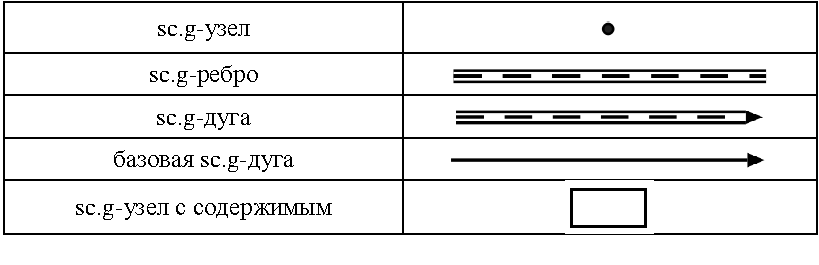
\includegraphics{figures/intro/SCg-core-alphabet.pdf}\\
}

%TODO сверить пропорции sc.g-элементов и изменить описание
\scnheader{sc.g-узел общего вида}
\scnidtf{\textit{sc.g-элемент}, являющийся графическим изображением \textit{sc-узла общего вида}}
\scnexplanation{Все \textit{sc-узлы}, не являющиеся знаками файлов, в тексте (конструкции) \textit{Ядра SCg-кода}, изображаются в виде небольших чёрных кругов одинакового радиуса, который обозначим через $\bm{r}$, и точная величина которого зависит от масштаба отображения \textit{sc.g-текста}.}

\scnheader{sc.g-ребро общего вида}
\scnidtf{\textit{sc.g-элемент}, являющийся графическим изображением \textit{sc-ребра общего вида}}
\scnexplanation{Каждое \textit{sc-ребро} в \textit{Ядре SCg-кода} изображается в виде линии произвольной формы, не имеющей самопересечений и имеющей толщину, равную примерно $\bm{r/8}$.}

\scnheader{sc.g-дуга общего вида}
\scnidtf{\textit{sc.g-элемент}, являющийся графическим изображением \textit{sc-дуги общего вида}}
\scnexplanation{Каждая \textit{sc-дуга} в \textit{Ядре SCg-кода} изображается в виде линии произвольной формы, не имеющей самопересечений, имеющей толщину равную $\bm{r/8}$ и имеющей изображение стрелочки на одном из концов этой линии.}

\scnheader{базовая sc.g-дуга}
\scnidtf{\textit{sc.g-элемент}, являющийся графическим изображением \textit{базовой sc-дуги}}
\scnexplanation{Каждая входящая в состав sc-текста \textit{базовая sc-дуга} в \textit{Ядре SCg-кода} изображается в виде линии произвольной формы, не имеющий самопересечений, имеющий толщину $\bm{r/4}$, и имеющей изображение стрелочки на одном из ее концов.}

\scnheader{внутренний файл ostis-системы}
\scnidtf{sc-узел с содержимым}
\scnaddlevel{1}
\scniselement{часто используемый sc-идентификатор}
\scnaddlevel{-1}
\scnidtf{sc-узел, являющийся знаком внутреннего файла ostis-системы}
\scnidtf{sc-знак внутреннего файла ostis-системы}

\scnheader{sc.g-узел с содержимым}
\scnidtf{sc.g-узел, имеющий содержимое}
\scnidtf{sc.g-узел, являющийся знаком внутреннего файла ostis-системы}
\scnidtf{sc.g-знак внутреннего файла ostis-системы}
\scnidtf{sc.g-рамка, ограничивающая изображение (представление) внутреннего файла ostis-системы, обозначаемого этой sc.g-рамкой}
\scnidtf{sc.g-рамка}
\scnaddlevel{1}
\scnnote{\textit{sc.g-рамка} -- это всегда прямоугольник, максимальный размер которого не ограничивается, но минимальный фиксируется и соответствует \textit{sc.g-рамке}, внутри которой обозначаемый ею \textit{файл} не отображается.}
\scnaddlevel{-1}
\scnexplanation{Каждый входящий в sc-текст \textit{sc-узел, имеющий содержимое}, в \textit{Ядре SCg-кода} изображается в виде прямоугольника произвольного размера с толщиной линии $\bm{r/6}$. Внутри этого прямоугольника отображается \textit{файл}, обозначаемый изображаемым \textit{sc-узлом}. Если нет необходимости изображать в тексте сам \textit{файл}, то \textit{sc-узел}, обозначающий такой \textit{файл}, в \textit{sc.g-тексте} изображается в виде прямоугольника со сторонами $\bm{2r}$ по вертикали и $\bm{4r}$ по горизонтали.}

\scnheader{Алфавит Ядра SCg-кода}
\scnnote{Трудно сразу поверить, что на основе такого простого алфавита можно построить удобный и \uline{универсальный} графовый язык. В рамках \textit{Документации Технологии OSTIS} мы постараемся Вас в этом убедить. Кроме того, нас не должна настораживать простота алфавита, поскольку человечество имеет большой опыт кодирования, хранения в памяти и передачи по каналам связи самых различных информационных ресурсов, используя алфавит, состоящий только из двух классов элементов -- единиц и нулей. 

Мы ведем речь о принципиально ином (графовом) способе кодирования информации в \textit{компьютерных системах}, но стараемся при этом свести это кодирование к достаточно простому алфавиту хотя бы для того, чтобы искусственно не усложнять проблему создания нового поколения компьютеров, основанных на указанном способе кодирования информации. 

Расширения \textit{Ядра SCg-кода} рассмотрим как направления перехода от текстов \textit{Ядра SCg-кода} к более компактным текстам. Но, поскольку это приводит к усложнению \textit{Синтаксиса SCg-кода} и, в первую очередь, к расширению \textit{Алфавита SCg-кода}, делать такие расширения необходимо обоснованно с учетом частоты встречаемости в рамках \textit{баз знаний ostis-систем} соответствующих фрагментов.}
\scnendstruct \scninlinesourcecommentpar{Завершили сегмент ``Описание Ядра SCg-кода''}

\scnsegmentheader{Описание Ядра SCg-кода}
\scnstartsubstruct

\scnfilelong{\textit{Алфавиту SC-кода} взаимно однозначно соответствует \textit{Алфавит Ядра SCg-кода} (алфавит \textit{sc.g-элементов}, графически изображающих \textit{sc-элементы}). Все \textit{sc-узлы}, не являющиеся знаками \textit{файлов}, в тексте (конструкции) \textit{Ядра SCg-кода} изображаются в виде небольших чёрных кругов одинакового радиуса, который обозначим через $r$, и точная величина которого зависит от масштаба отображения sc.g-текста. Каждое \uline{sc-ребро} в \textit{Ядре SCg-кода} изображается в виде линии произвольной формы не имеющий самопересечений и имеющей толщину, равную примерно $r/8$.

Каждая \uline{sc-дуга} в \textit{Ядре SCg-кода} изображается в виде линии произвольной формы, не имеющей самопересечений, имеющей толщину равную $r/8$ и имеющей изображение стрелочки на одном из концов этой линии. 

Каждая входящая в состав sc-текста \uline{базовая sc-дуга} в \textit{Ядре SCg-кода} изображается в виде линии произвольной формы, не имеющий самопересечений, имеющий толщину $r/4$, и имеющей изображение стрелочки на одном из ее концов. 

Каждый входящий в sc-текст \uline{sc-узел}, имеющий содержимое, в \textit{Ядре SCg-кода} изображается в виде прямоугольника произвольного размера с толщиной линии $r/6$. Внутри этого прямоугольника отображается \textit{файл}, обозначаемый изображаемым sc-узлом. Если нет необходимости изображать в тексте сам \textit{файл}, то sc-узел обозначающий такой файл в sc.g-тексте, изображается в виде прямоугольника со сторонами $2r$ по вертикали и $4r$ по горизонтали.

Таблицу соответствия между \textit{Алфавитом SC-кода} (Алфавитом абстрактных элементов sc-текстов) и \textit{Алфавитом Ядра SCg-кода} (Алфавитом графических примитивов, составляющих конструкции Ядра SCg-кода и являющихся изображениями sc-элементов). Смотрите в файле Таблица.Алфавит Ядра SCg-кода}

\scnsegmentheader{Описание Первого расширения Ядра SCg-кода}

\scnstartsubstruct

\bigskip
\scnfilelong{Первое расширения Ядра SCg-кода -- это уточнение типологии константных постоянных сущностей и расширение \textit{Алфавита Ядра SCg-кода}, позволяющее типологию \textit{константных постоянных сущностей} привести в соответствие с синтаксической типологией вводимых элементов \textit{Алфавита SCg-кода}. 

Понятие константы противопоставляется понятию переменной. Константа -- это знак конкретной фиксированный сущности, которая в текущий момент не обязательно должна быть детально изучена. Переменная -- это обозначение некоторой абстрактной произвольной сущности, которая может принимать ("пробегать") \uline{значения} из некоторого множества сущностей. 

Понятие постоянной сущности противопоставляется понятию временной сущности. \textit{Постоянная сущность} -- сущность, существующая \uline{всегда}. \textit{Временная сущность} -- сущность, существующая в течение некоторого отрезка времени. 

Рассмотрим подробнее sc.g-элементы, знаки \textit{константных постоянных сущностей} различного вида. Графическим признаком \textit{константных постоянных sc-узлов} в конструкциях SCg-кода является их изображение в виде \uline{окружностей} радиуса $2r$. Какое изображение является более компактной записью факта принадлежности заданного sc-узла (назовем его $\bm{vi}$) классу sc-констант и классу обозначений постоянных сущностей. Запись этого факта в \textit{Ядре SCg-кода} потребует (1) явного изображения sc-узла, обозначающего класс всевозможных константных sc-элементов (класс \textit{sc-констант}), (2) явного изображения базовой sc-дуги, соединяющего изображение sc-узла, обозначающего класс sc-констант, с изображением заданного константного sc-узла, (3) явного изображение sc-узла, обозначающего класс всевозможных sc-элементов, обозначающих \textit{постоянные сущности}, (4) явного изображения базовой sc-дуги, соединяющего изображение sc-узла, обозначающего класс обозначений \textit{постоянных сущностей} с изображением рассматриваемого sc-узла $\bm{vi}$ (\textit{Файл. Изображение спецификации sc.g-элемента средствами Ядра SCg-кода и Первого расширения Ядра SCg-кода}).

Общепринятая запись данного факта выглядит следующим образом:

"\textit{sc-константа} $\ni \bm{vi}$; \textit{постоянная сущность} $\ni \bm{v_i};$"

\textit{Константные постоянные sc-ребра} в конструкциях SCg-кода изображаются в виде двойной линии, каждая из которых имеет толщину $r/4$, а расстояние между ними также равно $r/4$. 

\textit{Константные постоянные sc-дуги} изображаются в виде такой же двойной линии, но со стрелочкой. Все базовые sc-дуги, а также все sc-узлы, имеющие содержимое, по определению являются \textit{константными постоянными sc-элементами}. 

\textit{Константные sc.g-узлы}, изображаемые окружностями радиуса $2r$, обозначают \textit{константные постоянные сущности}, о которых мало что известно, но известно то, что они не являются парами (то есть множествами, \textit{мощность*} которых равна 2) и, следовательно, не могут быть изображёны в виде sc.g-дуг или sc.g-рёбер. Но, если при этом об обозначаемой \textit{константной постоянной сущности} ($\bm{vi}$) известно, что она является классом сущностей, то текст *** можно заменить на более компактный ***. 

Аналогичным образом: 
\begin{scnitemize}
\item sc.g-текст *** означает, что некая сущность $\bm{vi}$ является \textit{отношением}; 
\item sc.g-текст *** означает, что некая сущность $\bm{vi}$ является \textit{ролевым отношением}; 
\item sc.g-текст *** означает, что некая сущность $\bm{vi}$ является \textit{небинарной связкой}; 
\item sc.g-текст *** означает, что некая сущность $\bm{vi}$ является \textit{структурой}; 
\item sc.g-текст *** означает, что некая сущность $\bm{vi}$ является первичный сущностью (терминальный сущностью, которая не является множеством, а также файлом, хранимым в памяти ostis-системы); 
\item sc.g-текст *** означает, что некая сущность $\bm{vi}$ является файлом, хранимым в памяти ostis-системы;
\item sc.g-текст *** означает, что некая сущность $\bm{vi}$ является файлом, хранимым в памяти ostis-системы, а знак этого файла обозначает также множество всевозможных его вхождений в другие файлы. 
\end{scnitemize}

Важное место среди константных постоянных сущностей занимают \textit{константные постоянные пары принадлежности}, обозначаемое соответствующими \textit{sc.g-дугами}. Такие пары принадлежности и обозначающие их sc.g-дуги бывают позитивными, негативными и нечеткими. Константная постоянная позитивная sc.g-дуга принадлежности есть ничто иное, как базовая sc.g-дуга. Константная постоянная негативная sc.g-дуга принадлежности изображается в виде "толстой"\ сплошной непунктирной линии со стрелкой и со штриховыми черточками. Константная постоянная нечёткая sc.g-дуга принадлежности изображается в виде толстой сплошной непунктирной линии со стрелкой и со штриховыми точками.}

\scnheader{Файл. Изображение спецификации sc.g-элемента средствами Ядра SCg-кода и Первого расширения Ядра SCg-кода}
\scneqfile{\\
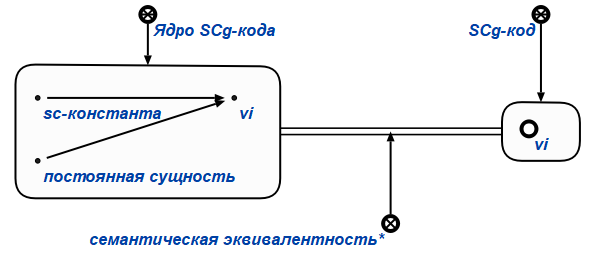
\includegraphics{figures/intro/scg1.png}\\
}
\scnendstruct

\scnsegmentheader{Описание Второго расширения Ядра SCg-кода}

\scnstartsubstruct

\bigskip
\scnfilelong{Второе расширение Ядра SCg-кода -- это расширение его алфавита путем введения дополнительных sc.g-элементов, обозначающих \textit{константные временные сущности} различного вида. Признаком sc.g-элементов, обозначающих \textit{константные временные сущности} являются точечные линии (линии, состоящие из точек, размер которых равен размеру изображаемой линии и которые близко расположены друг к другу на расстоянии, равном половине их размера), с помощью которых рисуются окружности при изображении sc-узлов, а также линии при изображении sc-коннекторов.

Результатом \textit{Второго расширения Ядра SCg-кода} является введение следующих видов sc.g-элементов (\textit{Таблица. sc.g-знаки константных временных сущностей}).
}

\scnheader{Таблица. sc.g-знаки константных временных сущностей}
\scneqfile{\\
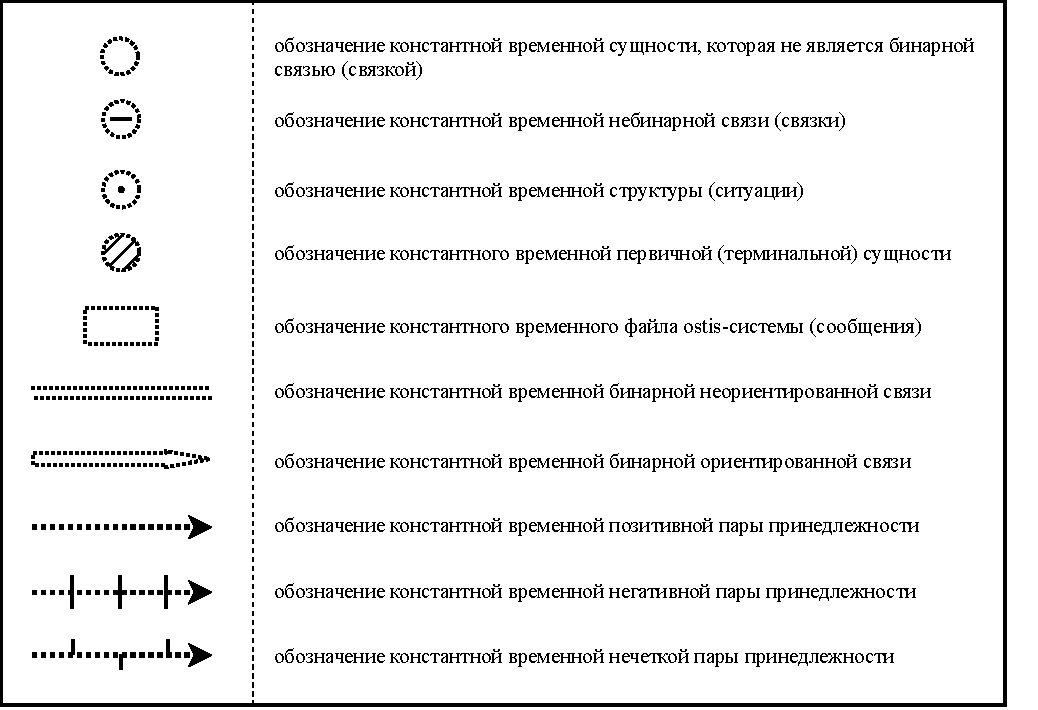
\includegraphics[width=1\linewidth]{figures/intro/SCg-temp-entities.pdf}\\
}

\scnendstruct

\scnsegmentheader{Описание Третьего расширения Ядра SCg-кода}

\scnstartsubstruct

\bigskip
\scnfilelong{Третья расширения ядра SCg-кода -- это расширение его алфавита путем введения дополнительных элементов, обозначающих \textit{переменные постоянные сущности} различного вида. Признаком sc.g-элементов, обозначающих сущности указанного класса, являются квадратики для изображения обозначений \textit{переменных постоянных сущностей}, не являющихся бинарными связями, а также пунктирные (в том числе и штрих-пунктирные) линии для изображения \textit{переменных постоянных бинарных связей}. 

Подчеркнем, что \textit{переменные постоянные сущности} могут отличаться друг от друга по характеру их \textit{области значений*}. Этими значениями в общем случае могут быть как \textit{константные постоянные сущности}, так и \textit{переменные постоянные сущности}. В любом случае, значение \textit{переменной сущности} является либо \textit{константной сущностью}, либо \textit{переменной сущностью}. Если каждое значение переменной является константой, то такую переменную будем называть \textit{переменной первого уровня}. Если каждое значение переменной является \textit{переменной первого уровня}, то такую переменную будем называть \textit{переменной второго уровня}. 

\textit{Переменная постоянная сущность первого уровня}, не являющаяся бинарной связью -- это переменная, каждым значением которой является \textit{константная постоянная сущность}, не являющаяся бинарной связью. Такая переменная изображается квадратиком, который ориентирован по вертикали и горизонтали. 

Указанная выше семантика такого изображения приписывается \uline{по умолчанию}. Это означает, что, если обозначаемая переменная имеет более сложную структуру области её значений, то эта область должна быть специфицирована явно. 

\textit{Переменная постоянная сущность второго уровня}, не являющаяся бинарной связью, изображается квадратиком, повернутым на 45$^\circ$.}

\scnheader{Таблица. sc.g-обозначения переменных постоянных сущностей}
\scneqfile{\\
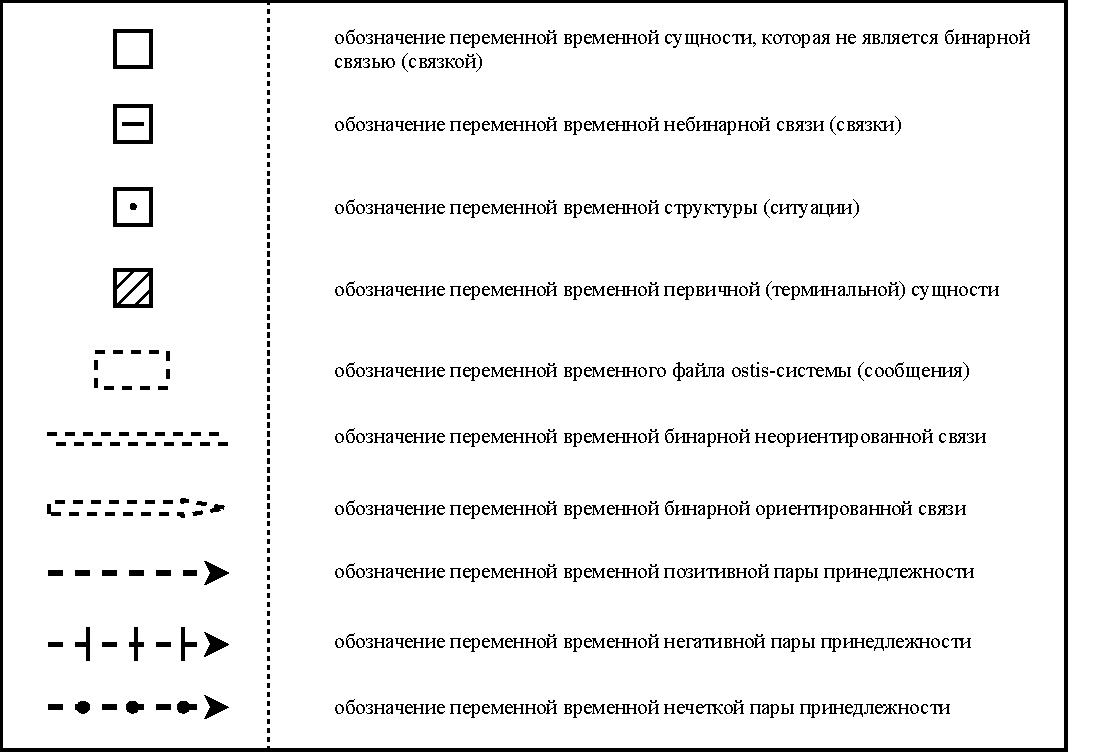
\includegraphics[width=1\linewidth]{figures/intro/SCg-var-entities.pdf}\\
}

\scnendstruct

\scnsegmentheader{Описание Четвертого расширения Ядра SCg-кода}

\scnstartsubstruct

\bigskip
\scnfilelong{Четвертое расширения Ядра SCg-кода -- это расширение его алфавита путем введения дополнительных sc.g-элементов, обозначающих \textit{переменные временные сущности} различного вида. Указанные дополнительные sc.g-элементы аналогичны тем, которые введены в рамках Второго расширения Ядра SCg-кода, и отличаются только тем, что в Четвёртом расширении Ядра SCg-кода речь идёт о переменных \uline{временных} сущностях, а во Втором расширении -- о переменных \uline{постоянных} сущностях.}

\scnendstruct

\scnsegmentheader{Описание Пятого расширения Ядра SCg-кода}

\scnstartsubstruct

\bigskip
\scnfilelong{Пятое расширение Ядра SCg-кода --  это приписывание некоторым sc.g-элементам \textit{основных внешних идентификаторов*} (чаще всего -- строковых идентификаторов, то есть имен) sc-элементов, изображаемых этими sc.g-элементами. Указанные идентификаторы являются уникальными для каждого идентифицируемого (именуемого) sc.g-элемента. Приписывание sc.g-элементам уникальных идентификаторов дает возможность в рамках одного sc.g-текста дублировать (копировать) некоторые sc.g-узлы при условии, если \uline{всем} таким копиям будут приписаны соответствующие идентификаторы. Такое дублирование sc.g-узлов является дополнительным средствам \uline{наглядного} размещения sc.g-текстов. 

Приписывание sc.g-элементу соответствующего ему основного (уникального) \textit{внешнего идентификатора*} представляет собой сокращённый вариант изображения sc.g-текстов, в которых приписывание идентификаторов отсутствует. Приведем пример. Пусть имеется некий sc.g-элемент, которому соответствует \textit{основной внешний идентификатор*} "$\bm{ei}$". Этот факт без переписывания указанного идентификатора указанному sc.g-элементу будет выглядеть следующим образом (\textit{Файл. Пример идентификации sc.g-элемента без использования средств Пятого расширения Ядра SCg-кода}). 

Здесь отношение, связывающее sc.g-элементы с файлами, содержащими их основные внешние идентификаторы, само имеет свой основной внешний идентификатор, который представляет собой строку символов, имеющую вид "основной внешний идентификатор*". Нетрудно заметить, что с помощью средства приписывания идентификаторов sc.g-элементам приведенная выше конструкция будет выглядеть тривиально: ***.}

\scnheader{Файл. Пример идентификации sc.g-элемента без использования средств Пятого расширения Ядра SCg-кода}
\scneqfile{\\
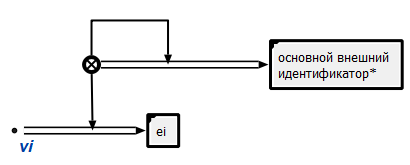
\includegraphics{figures/intro/scg2.png}\\
}

\scnendstruct

\scnsegmentheader{Описание Шестого расширения Ядра SCg-кода}

\scnstartsubstruct

\bigskip
\scnfilelong{\textbf{\textit{Шестое расширение Ядра SCg-кода}} -- это введение в SCg-код sc.g-контуров, sc.g-рамок и sc.g-шин как средств структуризации sc.g-текстов и повышения наглядности при их размещении. Подчеркнем, что и sc.g-контуры, и sc.g-шины, и sc.g-рамки являются специальными видами sc.g-элементов. При этом sc.g-контуры и sc.g-рамки являются sc.g-ограничителями (ограничителями SCg-кода).

Каждый sc.g-контур изображается (в 2D-модификации) в виде замкнутой ломаной линии, ограничивающей некоторый фрагмент sc.g-текста и обозначает множество всех \uline{sc-элементов}, sc.g-изображения которых оказались внутри этого контура.

Обозначение множества sc-элементов, изображаемое sc.g-контуром, может быть как константным, так и переменным. Соответственно этому линия, изображающая sc.g-контур может быть: 

\begin{scnitemize}
\item неточечной линией без пропусков,
\item точечной линией без пропусков,
\item неточечной пунктирной линией,
\item точечной пунктирной линией.
\end{scnitemize}

Семантическим эквивалентом sc.g-контуру является sc.g-узел, обозначающий sc-структуру. Использование sc.g-контура вместо указанного sc.g-узла исключает необходимость явно изображать SC-дуги принадлежности, выходящие из этого sc.g-узла. Это существенно повышает уровень наглядности sc.g-текста.

Если представленный внутри sc.g-контура текст не является sc.g-текстом, то считается, что что на самом деле внутренностью sc.g-контура является sc.g-текст, являющийся результатом переводя предоставленного текста в SCg-код.

Каждая sc.g-рамка является ограничителем изображения файла, обозначаемого этой sc.g-рамкой. Таким образом, sc.g-рамка может быть sc.g-ограничителем не только sc.g-текстов, но и любых других инородных для SCg-кода информационных конструкций, изображаемых на плоскости.

Семантическим эквивалентом sc.g-рамок являются sc.g-узлы следующего вида (\textit{Файл. Примеры SCg-рамок различного вида}).

Соответственно этому, sc.g-рамки всегда являются константными, хотя переменные, значениями которых являются sc.g-узлы, обозначающие файлы-ostis-систем, существуют, но  содержимого эти переменные иметь не могут.

Каждая sc.g-шина представляет собой замкнутую или незамкнутую линию, которая инцидентна только одному sc.g-элементу и семантически ему эквивалентна. Идея введения sc.g-шин заключается в увеличении «размеров» sc.g-элементов для расширения их области инцидентности. Особенно актуально это для sc.g-узлов, имеющих большое число инцидентных им sc.g-коннекторов.}

\scnheader{Файл. Примеры SCg-рамок различного вида}
\scneq{\scnfileshort{c.70}}

\scnendstruct

\scnsegmentheader{Описание Седьмого расширения Ядра SCg-кода}

\scnstartsubstruct

\bigskip
\scnfilelong{\textbf{\textit{Седьмое расширение Ядра SCg-кода}} -- это переход от 2D-изображений sc.g-текстов к 3D-изображениям.
Одним из вариантов трехмерного изображения sc.g-текстов является следующий:

\begin{scnitemize}
\item все sc.g-узлы изображаются, как и ранее, \uline{плоскими} графическими примитивами. При изменении точки просмотра они \uline{всегда} "поворачиваются"\ параллельно плоскости экрана, но их масштаб (размер на экране) при удалении от  точки просмотра \uline{уменьшается};
\item аналогичным "плоским"\ образом изображаются sc.g-рамки с их "внутренним"\ содержанием, а также внешние идентификаторы, приписываемые sc.g-элементам;
\item sc.g-коннекторы изображаются \uline{непересекающимися} линиями в трехмерном пространстве (заметим, что при изображении sc.g-текстов на плоскости пересечение sc.g-коннекторов часто снижает наглядность, "читательность"\ sc.g-текстов). Т.е. sc.g-коннекторы, которые на плоскости изображаются двойными линиями, в пространстве  цилиндрическими, "трубчатыми линиями"\ с находящейся внутри тонкой, но просвечивающейся осевой линией;
\item sc.g-контур в пространстве визуализируется несколькими (!) специального вида точками -- например там, где есть точки инцидентности sc.g-контура с \uline{внешними} sc.g-коннекторами. При этом sc.g-контур становится виден только по команде просмотра указываемого контура (указание контура – это указание одной из его точек инцидентности). По этой команде цветом выделяются все граничные точки контура (точки инцидентности) и все внутренние sc.g-элементы контура. Если просматривается  несколько контуров, то используется несколько цветов.
\end{scnitemize}

Вторым вариантом 3D-визуализации sc.g-текстов является размещение sc.g-текстов на параллельных плоскостях (слоях) с “прошивками”\ между этими слоями, соединяющими синонимичные sc.g-узлы, т.е. sc.g-узлы, имеющие одинаковые приписываемые им внешние идентификаторы. Такой вариант плоской, но многослойной визуализации sc.g-текстов дает возможность широко использовать те средства просмотра и редактирования sc.g-текстов, которые разработаны для плоской их визуализации.}

\scnendstruct

\scnsegmentheader{Последний сегмент Введения в SCg-код}

\scnstartsubstruct

\bigskip
\scnfilelong{Основная цель SCg-кода – иметь четкие синтаксические графические признаки изображения sc.g-элементов, позволяющие легко выделить и различать такие классы sc.g-элементов, как:

\begin{scnitemize}
\item sc.g-константы (знаки константных сущностей) и sc.g-переменные (изображения переменных, значениями которых являются соответсвующие sc.g-элементы);
\item sc.g-переменные, значениями которых являются константы, и sc.g-переменные, значениями которых являются переменные;
\item знаки постоянных (стабильных) сущностей и знаки временных (нестабильных, временно существующих, ситуативных) сущностей;
\item sc.g-коннекторы (знаки бинарных связей) и sc.g-элементы, не являющиеся sc.g-коннекторами;
\item неориентированные sc.g-коннекторы (sc.g-ребра) и ориентированные (sc.g-дуги);
\item sc.g-дуги принадлежности и sc.g-дуги, не являющиеся таковыми;
\item sc.g-дуги позитивной принадлежности, негативной принадлежности и нечеткой принадлежности.
\end{scnitemize}

Приведен перечень элементов Алфавита SCg-кода (см. Алфавит SCg-кода).
Этот перечень оформлен в виде sc.g-текста и представляет собой изображение примеров всех введенных видов sc.g-элементов (по одному примеру каждого вида). При этом, указанные примеры sc.g-элементов разбиты на пять групп (\textit{Текст SCg-кода. Алфавит SCg-элементов}). Первая группа (верхняя строка) включает в себя sc.g-элементы, для которых константность и постоянство обозначаемых ими сущностей требует дополнительного уточнения. Остальные четыре группы sc.g-элементов аналогичны друг другу и включают в себя соответственно:

\begin{scnitemize}
\item знаки \uline{константных постоянных} сущностей;
\item знаки \uline{константных временных} сущностей;
\item изображения переменных, значениями которых или значениями значений которых (в случае, если значениями переменных являются переменные) являются знаки константных \uline{постоянных} сущностей;
\item изображения переменных, значениями которых или значениями значений которых (в случае, если значениями переменных являются переменные) являются знаки константных \uline{временных} сущностей.
\end{scnitemize}

Особое место в Алфавите SCg-кода занимает графическое изображение SC-дуги принадлежности в виде сплошной непунктирной “толстой”\ линии со стрелкой и с размещенными на ней штрихованными точками и черточками.
Этот sc.g-элемент будем называть \textit{sc.g-дугой принадлежности}.
Данный sc.g-элемент используется тогда, когда нам необходимо изобразить SC-дугу, о которой известно, что она является SC-дугой принадлежности, но неизвестно о какой принадлежности идет речь -- о константной или переменной, о постоянной или временной, о позитивной, негативной или нечеткой.

Кроме sc.g-элементов, перечисленных в \textit{Текст SCg-кода. Алфавит SCg-кода}, в состав Алфавита SCg-кода входят также следующие sc.g-элементы:
\begin{scnitemize}
\item внешние идентификаторы sc.g-элементов, идентичные (приписываемые) сответствующим sc.g-элементам.
\item sc.g-контуры, каждый из которых является знаком некоторого sc-текста (структуры, состоящей из sc-элементов). Каждый такой sc-текст может быть:
\begin{scnitemizeii}
\item либо константной постоянной структурой (см. sc.g-элемент типа ***);
\item либо константной постоянной структурой (ситуацией) -- см. sc.g-элемент типа ***;
\item либо переменной структурой, значениями которой являются \uline{постоянные} структуры изоморфной  конфигурации (см. sc.g-элемент ***);
\item либо переменной структурой, значениями которой являются \uline{временные} структуры (ситуации) изоморфной  конфигурации (см. sc.g-элемент ***);
\end{scnitemizeii}

\item \textit{sc.g-рамки}, являющиеся ограничителями изображения различных файлов, хранимых в памяти ostis-системы (см. sc.g-элемент ***);
\item sc.g-шины, являющиеся обозначениями тех же сущностей, что и инцидентные им sc.g-элементы.
\end{scnitemize}

Заметим также, что, кроме всех перечисленных элементов Алфавита SCg-кода, каждый из которых имеет вполне определенную денотационную  семантику, для формализации синтаксиса SCg-кода необходимо ввести целый ряд более "мелких"\ синтаксических объектов, например:
\begin{scnitemize}
\item точек инцидентности sc.g-коннекторов с sc.g-узлами, с другими sc.g-коннекторами, с sc.g-контурами, с sc.g-рамками;
\item точек инцидентности sc.g-шин;
\item точек излома линейных sc.g-элементов (sc.g-коннекторов, sc.g-контуров, sc.g-рамок, sc.g-шин).
\end{scnitemize}
}

\scnheader{Текст SCg-кода. Алфавит SCg-кода}
\scneqfile{\\
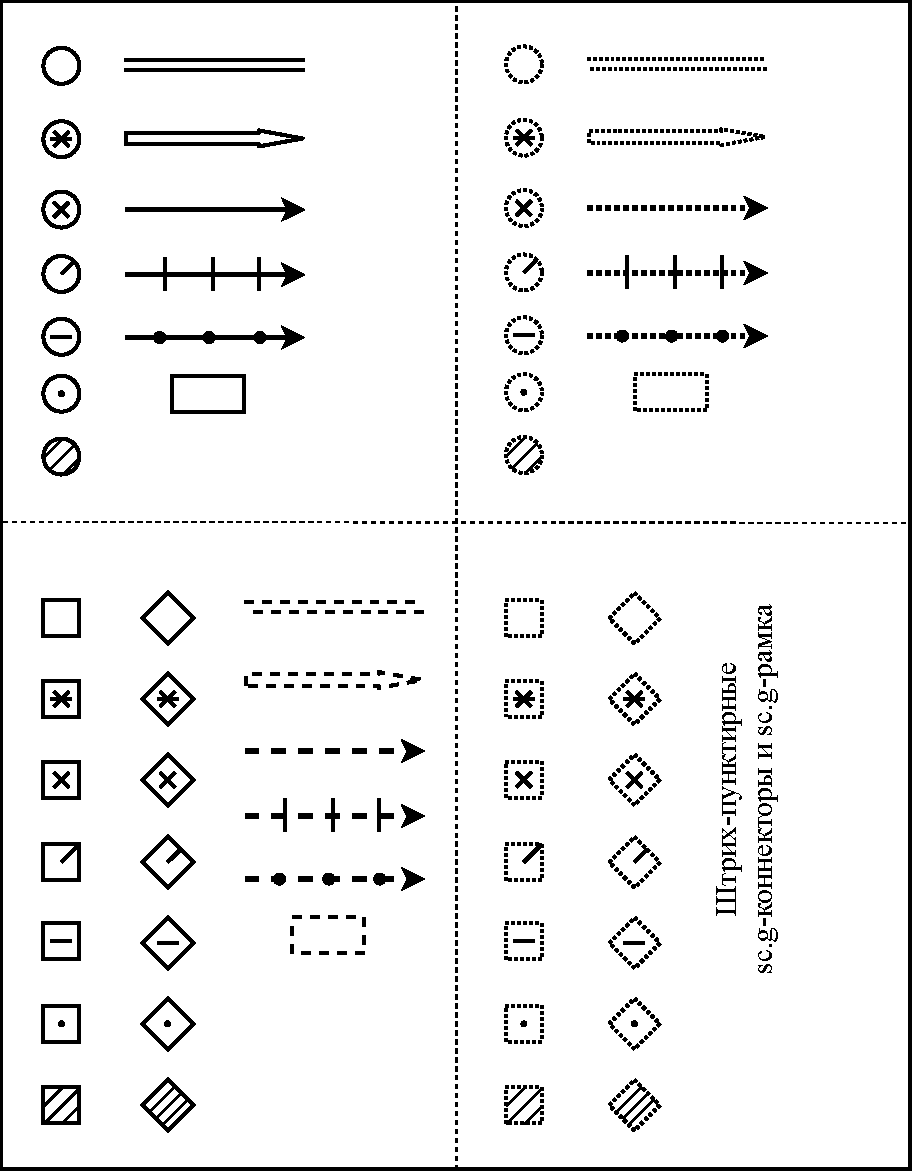
\includegraphics[width=1\linewidth]{figures/intro/SCg-full.pdf}\\
}


\scnendstruct

%End
\scnendstruct

\end{SCn}


\scsubsection{Введение в язык линейного представления баз знаний ostis-систем}
\label{intro_scs}

\begin{SCn}

\scnsectionheader{\currentname}

\scnstartsubstruct

\scnheader{Первый сегмент Введения в язык графического представления баз знаний ostis-систем}

\scnstartsubstruct

\scnheader{Введение в язык графического представления баз знаний ostis-систем}
\scnidtf{Введение в SCs-код}
\scnreltovector{конкатенация сегментов}{Первый сегмент Введения в SCs-код;Описание Алфавита SCs-кода;Описание sc.s-разделителей;Описание sc.s-ограничителей;Описание простых sc.s-идентификаторов;Описание sc.s-выражений;Описание sc.s-предложений;Описание Ядра SCs-кода и различных направлений его расширения}

\scnheader{SCs-код}
\scnidtf{Semantic Code string}
\scnidtf{Язык линейного представления баз знаний ostis-систем}
\scnidtf{Множество всевозможных текстов SCs-кода}
\scnidtf{Тексты SCs-кода}	
\scnaddlevel{1}
\scniselement{имя собственное}
\scnaddlevel{-1}
\scnidtf{текст SCs-кода}	
\scnaddlevel{1}
\scniselement{имя нарицательное}
\scnaddlevel{-1}
\scnidtf{sc.s-текст}
\scniselement{линейный язык}
\scnrelfrom{алфавит}{Алфавит SCs-кода}
\scnrelfrom{разделители}{sc.s-разделитель}
\scnrelfrom{ограничители}{sc.s-ограничитель}
\scnrelfrom{предложения}{sc.s-предложение}
\scnrelfrom{идентификаторы}{sc.s-идентификатор}
\scnrelfrom{неоднозначные обозначения описываемых сущностей}{неоднозначное sc.s-изображение sc-элемента}
\scnexplanation{Множество линейных текстов (sc.s-текстов), каждый из которых состоит из предложений (sc.s-предложений), разделенных друг от друга двойной точкой с запятой (разделителем sc.s-предложений). При этом sc.s-предложение представляет собой последовательность sc.s-идентификаторов, являющихся именами описываемых сущностей и разделяемых между собой различными sc.s-разделителями и sc.s-ограничителями}

\scnheader{sc.s-идентификатор}
\scnidtf{идентификатор, построенный по правилам SCs-кода}
\scnidtf{имя, построенное по правилам SCs-кода, обозначающее (идентифицирующее) соответствующую сущность, а так же одновременно идентифицирующее синонимичный этому имени sc-элемент, обозначающий ту же сущность, что и указанное имя}

\scnaddlevel{1}
	\scnidtf{строковый идентификатор}
	\scnsubset{идентификатор}
	\scnexplanation{обозначение описываемой сущности, структура которого в формальных языках однозначно соответствует этой сущности}
\scnaddlevel{-1}
\scnsubdividing{
простой sc.s-идентификатор\\
\scnaddlevel{1}
\scnidtf{атомарный sc.s-идентификатор}
\scnidtf{sc.s-идентификатор некоторого sc-элемента, в состав которого другие sc.s-идентификаторы (sc.s-идентификаторы других sc-элементов) не входят}
\scnidtf{простой (атомарный) внешний строковый идентификатор sc-элемента}
\scnaddlevel{-1}
;sc.s-выражение\\
\scnaddlevel{1}
\scnidtf{неатомарный sc.s-идентификатор}
\scnidtf{sc.s-идентификатор, представляющий собой в общем случае иерархическую конфигурацию sc.s-идентификаторов, связываемых между собой соответствующими sc.s-разделителями и sc.s-ограничителями}
\scnaddlevel{-1}
}

\scnheader{Неоднозначное sc.s-изображение sc-элемента}
\scnidtf{условное обозначение не именуемой (неидентифицируемой) сущности}
\scnsuperset{sc.s-коннектор}
\scnaddlevel{1}
    \scnidtf{неоднозначное sc.s-изображение sc-коннектора, являющееся также одновременно одним из видов sc.s-разделителей}
    \scnsubset{sc.s-разделитель}
\scnaddlevel{-1}
\scnsuperset{неоднозначное sc.s-изображение sc-узла}
\scnaddlevel{1}
    \scnsuperset{условное обозначение неименуемого множества sc-элементов}
    \scnaddlevel{1}
        \scnexplanation{условное обозначение неименуемого множества sc-элементов в SCs-коде представляется строкой из двух символов -- левой фигурной скобки и правой фигурной скобки. В SCs-коде, это соответствует кружочку с точкой внутри}
    \scnaddlevel{-1}
    \scnsuperset{условное обозначение неименуемого кортежа sc-элементов}
    \scnaddlevel{1}
        \scnexplanation{В SCs-коде такое обозначение представляется двух-символьной строкой левой угловой скобки и правой угловой скобки}
    \scnaddlevel{-1}
	\scnsuperset{условное обозначение неименуемого файла-экземпляра ostis-системы}
	\scnaddlevel{1}
		\scnexplanation{В SCs-коде такое обозначение представляется двух-символьной строкой левой квадратной скобки и правой квадратной скобки}
	\scnaddlevel{-1}
	\scnsuperset{условное обозначение не именуемого файла-класса ostis-системы}
	\scnaddlevel{1}
		\scnexplanation{В SCs-коде такое обозначение представляется трех-символьной строкой левой квадратной скобки, вертикальной черты (***), правой квадратной скобки}
	\scnaddlevel{-1}
\scnaddlevel{-1}
	
\scnendstruct

\scnheader{Описание Алфавита SCs-кода}
\scnstartsubstruct

\scnheader{Алфавит SCs-кода}
\scnidtf{Алфавит символов SCs-кода}
\scnidtf{множество символов SCs-кода}
\scnidtf{символ, используемый в текстах SCs-кода}
\scnreltoset{объединение}{символ, используемый в sc.s-разделителях;символ, используемый в sc.s-ограничителях;символ, используемый в простых sc.s-индетификаторах}

\scnheader{символ, используемый в sc.s-разделителях}
\scnhaselements{подчеркнутый пробел;дефис;запятая;пробел;точка;точка с запятой;двоеточие;“мячик”;знак равенства}
\scnhaselement{знак инцидентности правого sc-коннектора}
\scnaddlevel{1}
\scneqfile{/|-/}
\scnaddlevel{-1}
\scnhaselement{знак инцидентности левого sc-коннектора}
\scnaddlevel{1}
\scneqfile{/-|/}
\scnaddlevel{-1}
\scnhaselement{знак инцидентности входящей sc-дуги справа}
\scnaddlevel{1}
\scneqfile{/|</}
\scnaddlevel{-1}
\scnhaselement{знак инцидентности входящей sc-дуги слева}
\scnaddlevel{1}
\scneqfile{/>|/}
\scnaddlevel{-1}

\scnheader{символ, используемый в sc.s-разделителях}
\scnsuperset{символ, используемый в sc,s-коннекторах}
\scnaddlevel{1}
\scnhaselements{[/$\in$/];[/$\ni$/];[/$\notin$/];[/$\not \ni$/];[/***/];[/***/];[/$\sim$/];\textit{знак подчеркивания};\textit{знак тире};\textit{знак равенства};[/$\gt$/];[/$\gt$/];[/$\subseteq$/];[/$\supseteq$/];[/$\subset$/];[/$\supset$/];[/$\leq$/];[/$\geq$/];\textit{двоеточие}}
\scnaddlevel{-1}

\scnheader{символ, используемый в sc.s-разделителях}
\scnhaselement{вертикальная черта}
\scnhaselement{двойная вертикальная черта}
\scnaddlevel{1}
\scnidtf{знак операции конкатенации}
\scnaddlevel{-1}
\scnhaselement{знак операции объединения множеств}
\scnaddlevel{1}
\scnidtf{$\cup$}
\scnaddlevel{-1}
\scnhaselement{знак пересечения множеств}			\scnaddlevel{1}
\scnidtf{$\cap$}
\scnaddlevel{-1}
\scnhaselement{знак операции разности множеств}
\scnaddlevel{1}
\scnidtf{$\backslash$}
\scnaddlevel{-1}
\scnhaselement{знак операции сложения}	
\scnaddlevel{1}
\scnidtf{+}
\scnaddlevel{-1}
\scnhaselement{знак операции умножение}	
\scnaddlevel{1}
\scnidtf{*}
\scnaddlevel{-1}
\scnhaselement{знак операции вычитания}	
\scnaddlevel{1}
\scnidtf{‑}
\scnaddlevel{-1}

\scnheader{символ, используемый в sc.s-ограничителях}
\scnhaselement{прямые кавычки}
\scnaddlevel{1}
\scnidtf{"}
\scnaddlevel{-1}
\scnhaselement{левая круглая скобка}
\scnaddlevel{1}
\scnidtf{(}
\scnaddlevel{-1}
\scnhaselement{правая круглая скобка}
\scnaddlevel{1}
\scnidtf{)}
\scnaddlevel{-1}
\scnhaselement{левая фигурная скобка}
\scnhaselement{правая фигурная скобка}
\scnhaselement{левая угловая скобка}
\scnhaselement{правая угловая скобка}
\scnhaselement{левая квадратная скобка}
\scnhaselement{правая квадратная скобка}
\scnhaselement{косая черта}
\scnhaselement{звездочка вверху}
\scnhaselement{левая цитатная кавычка}
\scnhaselement{правая цитатная кавычка}

\scnheader{символ, используемый в простых sc.s-идентификаторах}
\scnsuperset{буква Русского языка}
\scnaddlevel{1}
\scnnote{и заглавная, и строчная}
\scnaddlevel{-1}
\scnsuperset{буква Английского языка}	\scnaddlevel{1}
\scnnote{и заглавная, и строчная}
\scnaddlevel{-1}
\scnsuperset{цифра}
\scnsuperset{спецсимвол, используемый в простых sc.s-идентификаторах}
\scnaddlevel{1}
\scneqtoset{знак подчеркивания;тире;дефис;запятая;	пробел;точка;двойная точка;прямая кавычка;звездочка вверху;крестик вверху;апостроф;круглая скобка}
\scnaddlevel{-1}

\scnendstruct \scnsourcecomment{Завершили Описание Алфавита SCs-кода}

\scnheader{Описание sc.s-разделителей}
\scnstartsubstruct

\scnheader{sc.s-разделитель}	\scnidtf{разделитель, используемый в sc.s-текстах}
\scnsubdividing{sc.s-разделитель, используемый в простых sc.s-идентификаторах;sc.s-разделитель, используемый в sc.s-выражениях\\
\scnaddlevel{1}
    \scnsuperset{точка с запятой}
    \scnaddlevel{1}
        \scnidtf{/;/}
    \scnaddlevel{-1}
    \scnsuperset{“мячик”}
    \scnaddlevel{1}
        \scnidtf{/$\bullet$/}
    \scnaddlevel{-1}
\scnaddlevel{-1}
;sc.s-разделитель, используемый для структуризации sc.s-предложений\\
\scnaddlevel{1}
    \scnsuperset{sc.s-коннектор}
    \scnsuperset{sc.s-разделитель, изображающий связь инцидентности sc-элементов}
    \scnsuperset{двоеточие}
    \scnaddlevel{1}
        \scnidtf{/:/}
        \scnnote{Разделяет ***}
    \scnaddlevel{-1}
\scnaddlevel{-1}
;sc.s-разделитель sc.s-предложений\\
\scnaddlevel{1}
    \scnidtf{/;;/}
    \scnidtf{/двойная точка с запятой/}
\scnaddlevel{-1}
}

\scnheader{sc.s-разделитель, используемый в простых sc.s-идентификаторах}
\scnsuperset{пробел}
\scnaddlevel{1}
    \scnnote{используется в качестве разделителя между словами, входящими в состав простого sc.s-идентификатора}
\scnaddlevel{-1}
\scnsuperset{подчеркнутый пробел}
\scnsuperset{запятая}
\scnaddlevel{1}
    \scnnote{используется в качестве разделителя между некоторыми словами, входящими в состав простого sc.s-идентификатора}
\scnaddlevel{-1}
\scnsuperset{точка}
\scnaddlevel{1}
    \scneqfile{/./}
    \scnnote{используется в конце аббревиатур, например, в инициалах}
\scnaddlevel{-1}
\scnsuperset{двойная точка}
\scnaddlevel{1}
    \scneqfile{/../}
    \scnnote{используется в качестве разделителя между содержательно разными частями простого sc.s-идентификатора, состоящего из нескольких фраз}
\scnaddlevel{-1}
\scnsuperset{двойная точка}
\scnaddlevel{1}
    \scneqfile{/-/}
    \scntext{примеры использования}{sc-текст; sc.s-разделитель}
\scnaddlevel{-1}

\scnheader{sc.s-коннектор}
\scnidtf{изображение sc-коннектора во внешнем тексте SCs-кода или SCn-кода}
\scnsubset{sc.s-разделитель}
\scnnote{типология sc.g-коннекторов и, тем более, sc-коннекторов, т.к. она она учитывает устоявшиеся традиции изображения связок целого ряда конкретных отношений}
\scnsubdividing{ориентированный sc.s-коннектор;неориентированный sc.s-коннектор}
\scnsubdividing{sc.s-коннектор, соответствующий sc.g-дуге принадлежности\\
\scnaddlevel{1}
    \scnrelfrom{таблица}{Таблица. Алфавит sc.s-коннекторов, соответствующих sc.g-дугам принадлежности}
\scnaddlevel{-1}
;sc.s-коннектор, соответствующий sc.g-коннектору, который не является sc.g-дугой принадлежности
\scnaddlevel{1}
    \scnrelfrom{таблица}{Таблица. Алфавит sc.s-коннекторов, соответствующих sc.g-коннекторам, которые не являются sc.g-дугами принадлежности}
\scnaddlevel{-1}
}

\scnheader{Таблица. Алфавит sc.s-коннекторов, соответствующих sc.g-дугам принадлежности}
\scneqfile{\\
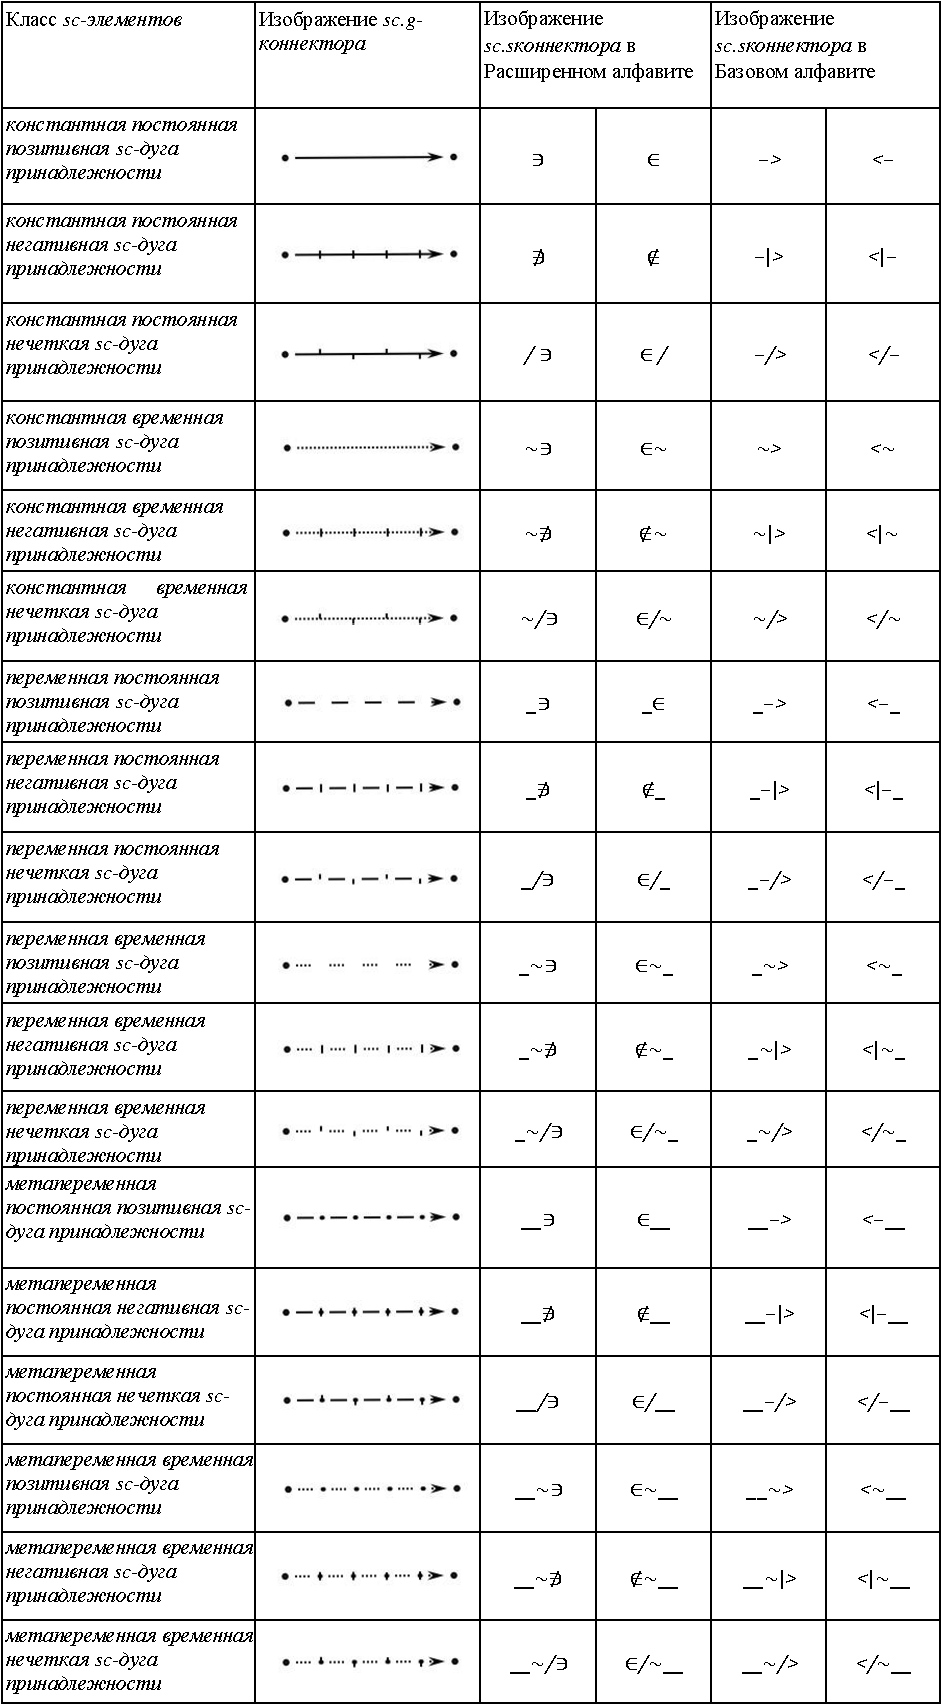
\includegraphics[width=1\linewidth]{figures/intro/scs_membership_connectors.pdf}\\
}

\scnheader{Таблица. Алфавит sc.s-коннекторов, соответствующих sc.g-коннекторам, которые не являются sc.g-дугами принадлежности}
\scneqfile{\\
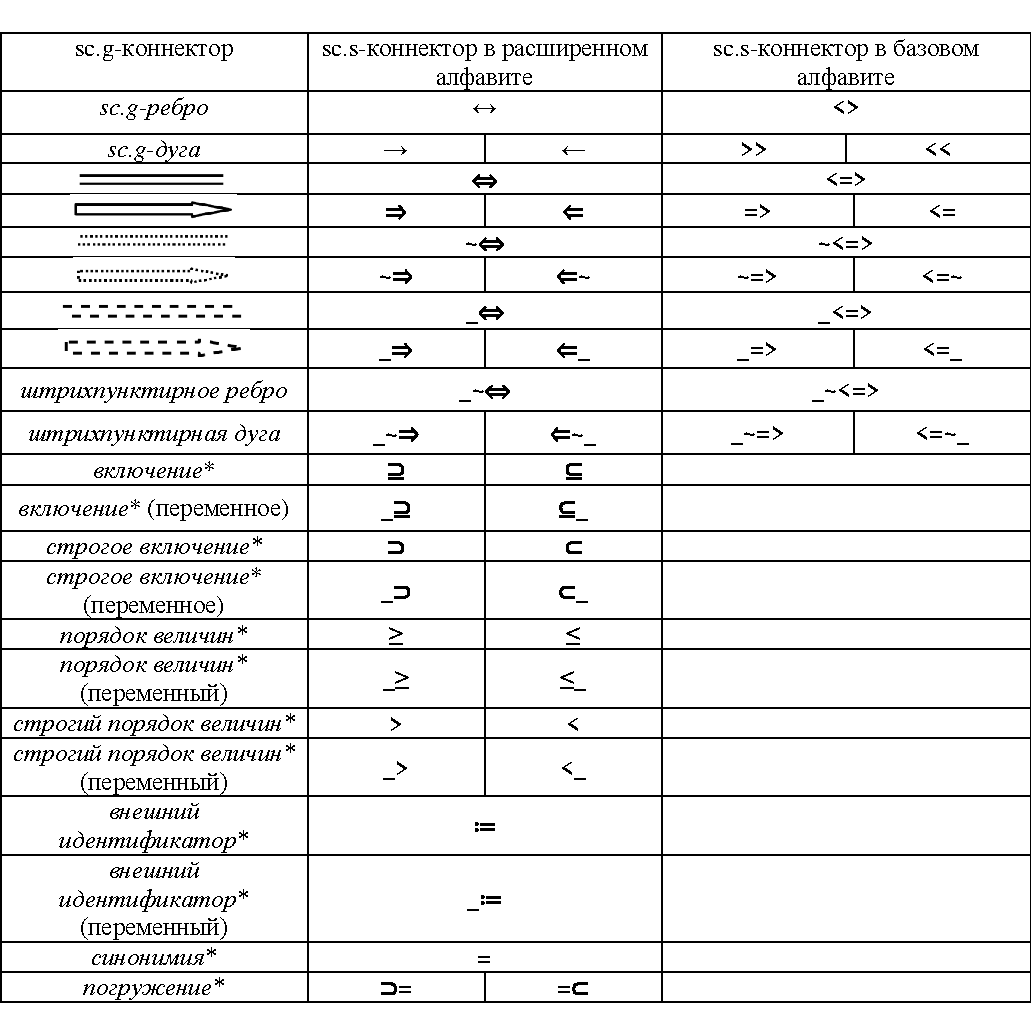
\includegraphics[width=1\linewidth]{figures/intro/scs_non_membership_connectors.pdf}\\
}

\scnheader{знак равенства}
\scneqfile{/=/}
\scnidtf{/связь синонимии идентификаторов/}
\scnnote{знак равенства является sc.s-разделителем двух sc.s-идентификаторов, которые идентифицируют (именуют) одну и ту же сущность и, соответственно, являются внешними идентификаторами* (внешними уникальными изображениями) одного и того же sc-элемента. При этом из указанных двух sc.s-идентификаторов чаще всего один является простым sc.s-идентификатором, а второй -- sc.s-выражением. Реже оба эти sc.s-идентификатора являются sc.s-выражениями. И совсем редко оба они являются простыми sc.s-идентификаторами. Последнее обозначает то, что оба эти sc.s-идентификатора являются основными внешними идентификаторами* одного и того же sc-элемента. Пример:

SC-код = sc.s-текст;;

Здесь первый sc.s-идентификатор является именем собственным, а второй -- именем нарицательным.

При трансляции sc.s-текста в SC-код знаку равенства на некотором этапе может быть поставлено в соответствие sc-ребро, принадлежащее отношению синонимии* sc-элементов, идентифицируемых sc.s-идентификаторами, связанными знаком равенства. Но на последующем этапе указанное sc-ребро \uline{удаляется}, а связанные им sc-элементы \uline{склеиваются}. Таким образом sc-ребро, принадлежащее отношению синонимии* sc-элементов, т.е. имеет не только денотационную, но и операционную семантику.}

\scnheader{знак равенства с включением}
\scneq{(\scnfileshort{/$\supset$=/} $\cup$ \scnfileshort{/=$\subset$/})}
\scnidtf{изображение sc-дуги, принадлежащей отношению погружения*, связывающей два sc-узла, обозначающих sc-тексты, первый из которых является погружающим, а второй (в который указанная sc-дуга входит) является погружаемым, вводимым в состав первого sc-текста}
\scnnote{sc-дуга, принадлежащая отношению погружения*, интерпретируется как команда погружения одного sc-текста в состав другого. При выполнении этой команды (1) все sc-элементы погружаемого sc-текста становятся элементами, принадлежащими погружающему sc-тексту, (2) все синонимичные sc-элементы, оказавшиеся в составе погружающего sc-текста, склеиваются, (3) sc-узел, обозначающий погружаемый sc-текст, а так же спецификация этого sc-текста (включая перечень всех его sc-элементов) погружается в историю эволюции базы знаний вместе со спецификацией события погружения рассматриваемого sc-текста в состав базы знаний.}

\scnheader{(знак равенства $\cup$ знак равенства с включением)}
\scnnote{указанные sc.s-коннекторы отличаются от остальных sc.s-коннекторов тем, что они и соответствующие им sc-коннекторы (sc-ребра, принадлежащих отношению синонимии sc-элементов и sc-дуги, принадлежащие отношению погружения одного sc-текста в состав другого) имеют не только денотационную, но и операционную семантику, т.к. являются командами склеивания и командами погружения.}

\scnheader{sc.s-разделитель, изображающий связь инцидентности sc-элементов}
\scnsubdividing{знак инцидентности “правого” sc-коннектора\\
\scnaddlevel{1}
\scnidtf{знак инцидентности sc-коннектора, sc.s-идентификатор которого находится справа}
\scneqfile{/|-/}
\scnaddlevel{-1}
;знак инцидентности “левого” sc-коннектора\\
\scnaddlevel{1}
\scnidtf{знак инцидентности sc-коннектора, sc.s-идентификатор которого находится слева}
\scneqfile{/-|/}
\scnaddlevel{-1}
;знак инцидентности входящей sc-дуги справа\\
\scnaddlevel{1}
\scnidtf{знак инцидентности sc-дуги, sc.s-идентификатор который находится справа}
\scneqfile{/|</}
\scnaddlevel{-1}
;знак инцидентности входящей sc-дуги слева\\
\scnaddlevel{1}
\scnidtf{знак инцидентности sc-дуги, sc.s-идентификатор который находится слева}
\scneqfile{/>|/}
\scnaddlevel{-1}}
\scnexplanation{На множестве sc-элементов задано бинарное ориентированное отношение инцидентности sc-элементов, а так же подмножество этого отношения -- отношение инцидентности входящих sc-дуг, каждая пара которого связывает sc-дугу с тем sc-элементом, в который она входит.
В SC-коде sc-коннекторы могут соединять между собой не только sc-узел с sc-узлами, но и sc-узел с sc-коннектором и даже sc-коннектор с sc-коннектором. В последнем случае, указывая инцидентность sc-коннекторов, необходимо уточнить, какой из них является соединяемым (связываемым), а какой-соединяющим (связующим). Поэтому отношение инцидентности, заданное на множестве sc-элементов является ориентированным. Первый компонент пары этого отношения -- связующий sc-коннектор, а второй -- связуемый sc-элемент. Очевидно, что связующий sc-элемент всегда является sc-коннектором, а sc-узел может быть только связуемым.}

\scnheader{sc.s-разделитель, изображающий связь инцидентности sc-элементов}
\scnnote{указанные sc.s-разделители с точки зрения синтаксической структуры sc.s-предложений аналогичны sc.s-коннекторам, но с точки зрения их денотационной семантики в отличие от sc.s-коннекторов они не являются изображениями соответствующих sc-коннекторов}

\scnendstruct \scnsourcecomment{Завершили Описание sc.s-разделителей}

\scnheader{Описание sc.s-ограничителей}
\scnstartsubstruct

\scnheader{sc.s-ограничитель}
\scnsubdividing{левый sc.s-ограничитель\\
    \scnaddlevel{1}
    \scnidtf{/ начальный sc.s-ограничитель /}
    \scnidtf{/ открывающий sc.s-ограничитель /}
    \scnaddlevel{-1}
;правый sc.s-ограничитель\\
    \scnaddlevel{1}
    \scnidtf{/ конечный sc.s-ограничитель /}
    \scnidtf{/ закрывающий sc.s-ограничитель /}
    \scnaddlevel{-1}}
\scnsubdividing{sc.s-ограничитель, используемый в простых sc.s-идентификаторах\\
    \scnaddlevel{1}
    \scnrelboth{пара пересекающихся множеств}{прямые кавычки}
        \scnaddlevel{1}
        \scneqfile{/"/}
        \scnidtf{/ограничитель метафорических словосочетаний/}
        \scnaddlevel{-1}
    \scnrelto{пара пересекающихся множеств}{круглая скобка}
        \scnaddlevel{1}
        \scneq{(\scnfileshort{/(/} $\cup$ \scnfileshort{/)/})}
        \scnaddlevel{-1}
    \scnnote{Данные ограничители используются не только в простых sc.s-идентификаторах: прямые кавычки — в нетранслируемых комментариях и в ея-файлах ostis-систем, а круглые скобки — везде (и в sc.s-выражениях, и в нетранслируемых комментариях, и в ея-файлах ostis-систем.}
    \scnaddlevel{-1}
;sc.s-ограничитель в sc.s-выражении;sc.s-ограничитель, используемый в sc.s-выражениях\\
    \scnaddlevel{1}
    \scnrelboth{пара пересекающихся множеств}{фигурная скобка}
    \scnaddlevel{1}
        \scneq{(\scnfileshort{/\{/} $\cup$ \scnfileshort{/\}/})}
        \scnexplanation{В sc.s-тексте фигурные скобки ограничивают sc.s-выражение, обозначающее либо множество sc-элементов, sc.s-идентификаторы которых перечисляются через точку с запятой, либо множество sc-элементов, входящих в состав sc-текста, который является результатом трансляции в SC-код sc.s-текста или даже ея-текста, ограниченного фигурными скобками.}
    \scnaddlevel{-1}
    \scnrelboth{пара пересекающихся множеств}{квадратная скобка}
        \scnaddlevel{1}
        \scnexplanation{В sc.s-тексте квадратные скобки ограничивают sc.s-выражение, обозначающее текстовый файл-экземпляр ostis-системы, содержимое (тело) которого изображается и ограничивается указанными квадратными скобками.}
        \scnaddlevel{-1}
    \scnrelboth{пара пересекающихся множеств}{квадратная скобка с вертикальной чертой}
        \scnaddlevel{1}
        \scnexplanation{В sc.s-тексте данный sc.s-ограничитель ограничивает sc.s-выражение, обозначающее текстовый файл-класс ostis-системы, содержимое (тело) которого изображается и ограничивается указанными sc.s-ограничителями.}
        \scnaddlevel{-1}
    \scnrelboth{пара пересекающихся множеств}{круглая скобка}
        \scnaddlevel{1}
        \scnexplanation{В sc.s-выражениях круглые скобки ограничивают перечень (через точку с запятой) sc.s-идентификаторов, обозначающих аргументы заданного квазибинарного ориентированного отношения, sc.s-идентификатор которого указывается перед левой круглой скобкой.}
        \scnaddlevel{-1}
    \scnaddlevel{-1}
;sc.s-ограничитель нетранслируемого комментария\\
    \scnaddlevel{1}
    \scnrelboth{пара пересекающихся множеств}{косая черта со звездочкой}
    \scnaddlevel{1}
        \scneq{(\scnfileshort{/ /* /} $\cup$ \scnfileshort{/ */ /})}
    \scnaddlevel{-1}
    \scnaddlevel{-1}
;sc.s-ограничитель, используемый в ея-файлах ostis-систем}

\scnsourcecomment{Завершили перечень видов sc.s-ограничителей}

\scnendstruct \scnsourcecomment{Завершили Описание sc.s-ограничителей}

\scnheader{Описание простых sc.s-идентификаторов}
\scnstartsubstruct

\scntext{правила построения}{Правила построения простых sc.s-идентификаторов.\\
Данные правила включают в себя:
\begin{scnitemize}
    \item Символы, используемые в простых sc.s-идентификаторах (в том числе, специальные символы);
    \item Специальные предикаты, используемые в простых sc.s-идентификаторах;
    \item Специальные суффиксы, используемые в простых sc.s-идентификаторах;
    \item Разделители, используемые в простых sc.s-идентификаторах;
    \item Ограничители, используемые в простых sc.s-идентификаторах;
    \item Правила построения простых sc.s-идентификаторов, определяемые различными классами идентифицируемых сущностей;
    \item Правила построения sc.s-имен собственных и sc.s-имен нарицательных.
\end{scnitemize}
Общим правилом построения простых sc.s-идентификаторов является стремление максимально возможным образом использовать сложившуюся терминологию. Но при этом следует подчеркнуть, что необходимость исключения омонимии в sc.s-идентификаторах требует строгого формального \uline{уточнения} семантической интерпретации каждого используемого термина. Особо подчеркнем то, что в ostis-системах процесс построения новых терминов (sc.s-идентификаторов) и процесс совершенствования существующей терминологии по отношению к процессу развития ostis-систем, баз знаний, представленных в SC-коде, с технической точки зрения абсолютно не зависят друг от друга. Кроме того, следует помнить, что \uline{далеко не все} sc-элементы, входящие в состав базы знаний ostis-системы, должны иметь соответствующие им sc.s-идентификаторы (быть идентифицированными). Очевидно, что идентифицированными (именованными) должны быть все используемые понятия, вводимые в соответствующих предметных областях и специфицируемые соответствующими онтологиями. Идентифицированными также должны быть обладающие особыми свойствами ключевые экземпляры (элементы) некоторых понятий, различные социально значимые объекты (персоны, населенные пункты, географические объекты, страны, организации, библиографические источники и многое другое).\\
Рассмотрим правила построений простых sc.s-идентификаторов, определеяемые различными классами идентифицируемых сущностей:
\begin{scnitemize}
    \item Первым символом каждого простого sc.s-идентификатора и каждого sc.s-выражения, идентифицирующего sc-переменную (переменный sc-элемент), является подчеркнутый пробел;
    \item Последним символом простого sc.s-идентификатора, идентифицирующего sc-узел, обозначающий неролевое отношение, заданное на множестве sc-элементов, является крестик в виде верхнего индекса;
    \item Последним символом простого sc.s-идентификатора, идентифицирующего sc-узел, обозначающий заданное на множестве sc-элементов ролевое отношение (т.е. отношение, являющееся подмножеством отношения принадлежности), является апостроф (черточка в виде верхнего индекса);
    \item Последним символом простого sc.s-идентификатора, идентифицирующего sc-узел, обозначающий понятие, не являющееся отношением, (таковыми, в частности, являются различного рода параметры — длина, площадь, объем, масса) является звездочка в виде верхнего индекса;
    \item В рамках SCs-кода целесообразно вводить правила унифицированного построения простых sc.s-идентификаторов и целого ряда других классов идентифицируемых сущностей — персон, библиографических источников (публикаций), разделов баз знаний ostis-систем, файлов ostis-систем, самих ostis-систем.
\end{scnitemize}}

\scnheader{имя нарицательное}
\scnidtf{имя, которое может быть приписано \uline{любому} экземпляру некоторого класса и которое обозначает указаный класс}
\scntext{примеры}{треугольник; город; персона; отношение; параметр; константа; переменная}
\scnnote{имя собственное в SCs-коде всегда начинается с маленькой буквы}

\scnheader{имя собственное}
\scnidtf{имя, которое либо не является обозначением какого-либо класса сущностей, либо является обозначением (именем) некоторого класса сущностей, но построенным без использования нарицательного имени этого класса, либо является именем некоторого класса сущностей, построенным с использованием нарицательного имени этого класса (1) путем преобразования имени нарицательного во множественное число или (2) путем дополнительного использования в начале формируемого имени собственнного таких терминов, как ``Класс...'', ``Множество...'', ``Множество всевозможных...''.}
\scntext{примеры}{Москва; Иванов Иван Сергеевич; Точка А; Город Минск; SC-код; Русский язык; Множество всевозможных sc-текстов; Класс sc-текстов; Класс русскоязычных текстов.}
\scnnote{имя собственное в SCs-коде всегда начинается с большой буквы}

\scnendstruct \scnsourcecomment{Завершили Описание sc.s-идентификаторов}


\scnsectionheader{Описание sc.s-выражений}
\scnstartsubstruct

\scnheader{sc.s-выражение}
\scnsuperset{sc.s-выражение, идентифицирующее sc-коннектор}
\scnsuperset{sc.s-выражение, ограничиваемое фигурными скобками и обозначающее множество sc-элементов, все sc.s-идентификаторы которых перечисляются}
\scnsuperset{sc.s-выражение, ограничиваемое фигурными скобками и обозначающее множество sc-элементов, входящих в состав sc-текста, который семантически эквивалентен тому sc.s-тексту или ея-тексту, который ограничен указанными фигурными скобками}
\scnsuperset{sc.s-выражение, ограничиваемое квадратными скобками и обозначающее файл-экземпляр ostis-системы}
    \scnaddlevel{1}
    \scnrelfrom{смотрите}{Принципы SC-кода}
        \scnaddlevel{1}
        \scniselement{секция раздела базы знаний}
        \scnaddlevel{-1}
    \scnaddlevel{-1}
\scnsuperset{sc.s-выражение, ограничиваемое квадратными скобками и дополнительными вертикальными линиями (или кавычками) и обозначающее файл-класс ostis-системы}
    \scnaddlevel{1}
    \scnrelfrom{смотрите}{Принципы SC-кода}
        \scnaddlevel{1}
        \scniselement{секция раздела базы знаний}
        \scnaddlevel{-1}
    \scnaddlevel{-1}
\scnsuperset{sc.s-выражение, использующее знаки алгебраических операций}
    \scnaddlevel{1}
    \scntext{примеры}{($s_i \cup s_j \cup s_k$); ($s_i \cap s_j \cap s_k$); ($s_i \backslash s_j$); ($x+y+z$); ($x \times y \times z$)}
    \scnaddlevel{-1}
\scnsuperset{sc.s-выражение, обозначающее второй компонент пары указываемого ориентированного бинарного или квазибинарного отношения для указываемых аргументов\\
    \scnaddlevel{1}
    \scntext{примеры}{объединение*($s_i$; $s_j$; $s_k$); пересечение*($s_i$; $s_j$; $s_k$); разность множеств*($s_i$; $s_j$); сложение*($x$; $y$; $z$); умножение*($x$; $y$; $z$); sin*($x$); cos*($x$)}
    \scnaddlevel{-1}}
\scnexplanation{Использование sc.s-выражений позволяет существенно сократить число "придумываемых" sc.s-идентификаторов, каковыми в конечном счете становятся только простые sc.s-идентификаторы, поскольку, зная то, как связан идентифицируемый sc-элемент с теми sc-элементами, которые уже имеют sc.s-идентификаторы, во многих случаях можно построить sc.s-выражение, идентифицирующее указанный sc-элемент. Кроме того, каждое sc.s-выражение, являясь внешним идентификатором, является также и \uline{транслируемым} формальным текстом, содержащим некоторую информацию об обозначаемой ею сущности.}

\scnheader{sc.s-выражение, идентифицирующее sc-коннектор}
\scnnote{Поскольку кратные sc-коннекторы одного и того же вида встречаются редко, sc.s-выражение, идентифицирующее sc-коннектор, чаще всего \uline{однозначно} идентифицирует соответствующий sc-коннектор. В случае кратных sc-коннекторов одинакового семантического вида, отражаемого типом sc.s-коннектора, можно, например, sc.s-выражениям, идентифицирующим разные кратные sc-коннекторы, приписывать разные номера. Пусть, например, sc-элементы $e_i$ и $e_j$ соединены двумя \uline{кратными} константными постоянными sc-дугами. Тогда указанные sc-дуги можно идентифицировать следующими sc.s-выражениями:\\
($e_i => e_j$)1\\
($e_i => e_i$)2\\}

\scnheader{Файл-рисунок на странице 125}
\scnexplanation{В данном файле ostis-системы приведено определение понятия sc.s-выражения, идентифицирующего sc-коннектор, представленное в SCg-коде и на Языке Бэкуса-Наура*.}

\scnheader{Таблица.Типология sc.s-выражений}
\scneqfile{\\
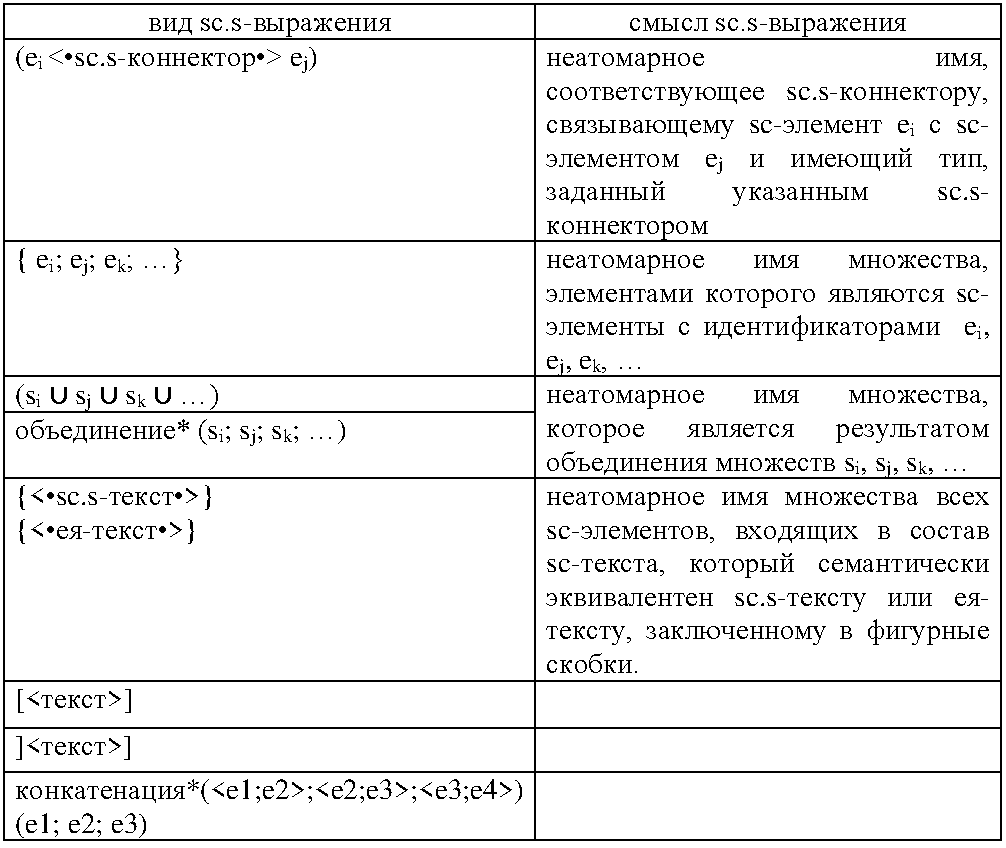
\includegraphics[width=1\linewidth]{figures/intro/scs-statements.pdf}\\
}

\scnendstruct \scnsourcecomment{Завершили Описание sc.s-выражений}

\scnheader{Описание sc.s-предложений}
\scnstartsubstruct

\scnheader{sc.s-предложение}
\scnidtf{минимальный семантически целостный фрагмент sc.s-текста}
\scnidtf{минимальный sc.s-текст}
\scnsubset{sc.s-текст}
\scnsuperset{простое sc.s-предложение\\
    \scnaddlevel{1}
    \scnidtf{sc.s-предложение, \uline{состоящее} из двух sc.s-идентификаторов, соединенных между собой sc.s-коннектором или sc.s-разделителем, изображающим связь инцидентности sc-элементов, и завершающееся двойной точкой с запятой}
    \scnaddlevel{-1}}
\scnnote{Признаком завершения любого sc.s-предложения, т.е. последними его символами является двойная точка с запятой, которую, следовательно можно считать разделителем sc.s-предложений.}
\scnrelfromlist{заданная операция}{Операция конверсии sc.s-предложения\\
    \scnaddlevel{1}
    \scnexplanation{Каждое sc.s-предложение (в том числе, и простое sc.s-предложение) можно преобразовать в семантически эквивалентное ему sc.s-предложение путем конверсии (``разворота'') цепочки компонентов sc.s-предложения. Так, например, при конверсии (``развороте'') простого sc.s-предложения (1) первый его sc.s-идентификатор (первый компонент этого sc.s-предложения) становится третьим компонентом конвертированного sc.s-предложения, (2) второй его sc.s-идентификатор (третий компонент исходного sc.s-предложения) становится первым компонентом ``конвертированного'' sc.s-предложения и (3) второй компонент исходного sc.s-предложения (sc.s-коннектор или sc.s-разделитель, изображающий связь инцидентности sc-элементов, соединяющий указанные выше компоненты) остается вторым компонентом конвертированного sc.s-предложения, но меняет направленность (``$\ni$'' заменяется на ``$\in$'' и наоборот, ``$\supset$'' на ``$\subset$'' и наоборот, ``$=>$'' на ``$<=$'' и наоборот и т.д.)}
    \scnnote{Можно говорить не только о конверсии sc.s-предложения, но и о конверсии sc.s-коннектора, о конверсии sc.s-разделителя, изображающего связь инцидентности sc.s-элементов.}
    \scnaddlevel{-1}
;Операция соединения двух sc.s-предложений при совпадении последнего компонента первого предложения с первым компонентом второго\\
    \scnaddlevel{1}
    \scnexplanation{В результате выполнения данной операции два исходных sc.s-предложения соединяются в одно sc.s-предложение путем ``склеивания'' указанных совпадающих компонентов и удаления двойной точки с запятой, разделяющей исходные два предложения.}
    \scnaddlevel{-1}
;Операция присоединения простого sc.s-предложения к sc.s-предложению, у которого последний sc.s-коннектор совпадает с sc.s-коннектором простого sc.s-предложения, а предшествующий указанному sc.s-коннектору sc.s-идентификатор совпадает с первым sc.s-идентификатором простого sc.s-предложения\\
    \scnaddlevel{1}
    \scnexplanation{В результате выполнения этой операции совпадающие sc.s-идентификаторы и sc.s-коннекторы соединяемых sc.s-предложений ``склеиваются'', а последние sc.s-иден\-ти\-фи\-ка\-то\-ры соединяемых sc.s-предложений становятся последними компонентами объединенного sc.s-предложения,
    разделенными точкой с запятой. Аналогичным образом можно присоединять сколько угодно простых sc.s-предложений.}
    \scnaddlevel{-1}
;Операция разложения sc.s-предложений на простые sc.s-предложения\\
    \scnaddlevel{1}
    \scnexplanation{Каждое sc.s-предложение можно разложить на множество простых sc.s-предложений, т.е. представить в виде последовательности простых sc.s-предложений}
    \scnaddlevel{-1}
;Операция разложения sc.s-предложений на простые sc.s-предложения с sc.s-разделителем, изображающим связь инцидентности sc-элементов\\
    \scnaddlevel{1}
    \scnexplanation{Каждое sc.s-предложение (в том числе и простое sc.s-предложение с sc.s-коннектором) можно представить в виде семантически эквивалентной последовательности простых sc.s-предложений с sc.s-разделителем, изображающим связь инцидентности sc-элементов.}
    \scnnote{Данная операция осуществляет \uline{однозначное} (!) формирование множества простых sc.s-предложений указанного вида.}
    \scnaddlevel{-1}
    }

\scnheader{sc.s-предложение}
\scnnote{Операции, заданные на множестве sc.s-предложений можно разделить на три группы:
    \begin{scnitemize}
        \item группа операций конверсии sc.s-предложений, состоящая из одной операции;
        \item группа операций соединения sc.s-предложений;
        \item группа операций декомпозиции sc.s-предложений и, в частности, операций разложения sc.s-предложений.
    \end{scnitemize}
Очевидно, что операции соединения sc.s-предложений и операции декомпозиции sc.s-предложений являются обратными друг другу операциями.}

\scnheader{компонент sc.s-предложения*}
\scnexplanation{Каждое sc.s-предложение представляет собой последовательность (1) sc.s-идентификаторов, (2) sc.s-коннекторов или sc.s-разделителей, изображающих связь инцидентности sc-элементов, (3) точек с запятыми, завершаемая двойной точкой с запятой. При этом непосредственно соседствовать друг с другом не могут ни sc.s-идентификаторы, ни sc.s-коннекторы, ни, очевидно, точки с запятыми.\\
Между sc.s-идентификаторами в рамках sc.s-предложения может находиться либо точка с запятой, либо sc.s-коннектор, либо sc.s-разделитель, изображающий связь инцидентности sc-элементов. Слева и справа от sc.s-коннектора и от sc.s-разделителя, изображающего связь инцидентности sc-элементов, должны находиться sc.s-идентификаторы.

Указанные sc.s-идентификаторы, sc.s-коннекторы и sc.s-разделители, изображающие связь инцидентности sc-элементов, считаются компонентами соответствующего sc.s-предложения. Понятие ``быть компонентом sc.s-предложения'' является относительным понятием (отношением), т.к. в состав некоторых компонентов sc.s-предложения (в состав sc.s-идентификаторов, являющихся sc.s-выражениями, ограничиваемыми фигурными или квадратными скобками) могут входить других sc.s-предложения, состоящие из своих компонентов.}
    
\scnheader{sc.s-предложение}
\scntext{денотационная семантика}{С семантической точки зрения sc.s-предложение представляет собой описание некоторого \uline{маршрута} в соответствующем sc-тексте, который является графовой структурой специального вида и структура которого описывается (изображается) с помощью sc.s-предложений. Указанный маршрут ``проводится'' по sc-коннекторам и по связям инцидентности sc-элементов, если маршрут проходит через инцидентные sc-коннекторы. В описании указанного маршрута могут дополнительно указываться множества (чаще всего отношения), которым принадлежат sc-коннекторы, входящие в описываемый маршрут. Кроме того, указанный маршрут в начале и/или в конце может иметь разветвления, когда какой-либо sc-элемент \uline{одинаково} инцидентен нескольким \uline{однотипным} sc-коннекторам, соединяющим указанный sc-элемент с некоторыми другими sc-элементами.

Таким образом каждое указанное разветвление состоит из неограниченного числа ветвей, каждая из которых состоит из одного sc-коннектора и одного связываемого им sc-элемента.}

\scnheader{sc.s-модификатор*}
\scnsubset{компонент sc.s-предложения*}
\scnexplanation{Это дополнительный вид компонентов sc.s-предложений. Каждый sc.s-модификатор, являющийся компонентом некоторого sc.s-предложения, представляет собой sc.s-идентификатор, обозначающий множество (чаще всего, отношение), которому принадлежит sc-коннектор, изображенный sc.s-коннектором, который предшествует указанному sc.s-идентификатору. Признаком sc.s-модификатора является двоеточие, которое ставится после sc.s-модификатора и отделяет его либо от следующего за ним другого sc.s-модификатора для этого же sc.s-коннектора, либо от следующего за ним sc.s-идентификатора, соответствующего sc-элементу, который инцидентен sc-коннектору, изображенному sc.s-коннектором, находящимся левее рассматриваемого sc.s-идентификатора после одного или нескольких sc.s-модификаторов.}

\scnheader{sc.s-текст}
\scnidtf{конкатенация sc.s-предложений}
\scnidtf{последовательность sc.s-предложений, разделяемых двойными точками с запятой}
\scnsuperset{максимальный исходный sc.s-текст}
    \scnaddlevel{1}
    \scnidtf{конкатенция sc.s-предложений, слева и справа от которой отсутствуют какие-либо символы SCs-кода}
    \scnaddlevel{-1}
\scnsuperset{максимальный встроенный sc.s-текст}
    \scnaddlevel{1}
    \scnidtf{конкатенция всех sc.s-предложений, входящих в состав sc.s-выражения, ограничиваемого фигурными скобками}
    \scnaddlevel{-1}
\scnsuperset{исходный sc.s-текст}
    \scnaddlevel{1}
    \scnidtf{часть цепочки sc.s-предложений, входящих в состав максимального исходного sc.s-текста}
    \scnsuperset{исходное sc.s-предложение}
    \scnaddlevel{-1}
\scnsuperset{встроенный sc.s-текст}
    \scnaddlevel{1}
    \scnidtf{часть цепочки sc.s-предложений, входящих в состав максимального встроенного sc.s-текста}
    \scnsuperset{встроенное sc.s-предложение}
    \scnaddlevel{-1}
\scnnote{sc.s-предложение является минимальным sc.s-текстом.}
\scntext{свойство}{Смысл исходного sc.s-текста, а также встроенного sc.s-текста независит от порядка sc.s-предложений в этих sc-текстах. Т.е. перестановка sc.s-предложений в рамках таких sc.s-текстов смысла этих sc.s-текстов не меняет (т.е. приводит к семантически эквивалентным sc.s-текстам), но сильно влияет на трудоемкость человеческого восприятия (на ``читабельность'') этих текстов.}

\scnendstruct \scnsourcecomment{Завершили Описание sc.s-предложений}

\scnheader{Описание Ядра SCs-кода и различных направлений его расширения}
\scnstartsubstruct

\scnheader{Ядро SCs-кода}
\scnidtf{Подъязык SCs-кода, который использует минимальный набор семантических средств, но при этом имеет семантическую мощность, эквивалентную мощности SCs-кода в целом}
\scntext{принципы}{В Ядре SCs-кода:
\begin{scnitemize}
    \item используются только простые sc.s-идентификаторы (sc.s-выражения не используются);
    \item используются только sc.s-разделители, изображающие связь инцидентности sc-элементов (sc.s-коннекторы не используются);
    \item не используются sc.s-модификаторы и, соответственно, двоеточия, являющиеся признаком завершения sc.s-модификаторов;
    \item используются только простые sc.s-предложения, которые, как следует из вышеуказанных свойств Ядра SCs-кода, состоят из двух простых sc.s-идентификаторов, соединяемых sc.s-разделителем, изображающим связь инцидентности sc-элементов.
\end{scnitemize}

Из перечисленных свойств Ядра SCs-кода следует, что для представления (изображения) любого sc-текста средствами Ядра SCs-кода необходимо для \uline{всех} (!) sc-элементов этого sc-текста построить соответствующие им простые sc.s-идентификаторы, т.е. необходимо проименовать все указанные sc-элементы.}
\scntext{примечание}{Очевидно, что практического значения Ядро SCs-кода не имеет. Для обеспечения возможности практического использования необходимы синтаксические расширения Ядра SCs-кода в целях:
\begin{scnitemize}
    \item минимизации числа идентифицируемых (именуемых) sc-элементов путем введения sc.s-выражений и ликвидации необходимости идентифицировать (именовать) \uline{все} (!) sc-элементы;
    \item сокращения текста путем минимизации числа повторений одного и того же sc.s-идентификатора путем соединения sc.s-предложений;
    \item повышение уровня наглядности, ``читабельности'' sc.s-текстов.
\end{scnitemize}}

\scnheader{Первое направление расширения Ядра SCs-кода}
\scnidtf{Первое направление расширения Ядра SCs-кода \uline{и всех иных его расширений}}
\scntext{принципы}{По сравнению с Ядром SCs-кода в Первом направлении расширения Ядра SCs-кода вместо sc.s-идентификаторов, являющихся идентификаторами (именами), которые взаимно однозначно соответствуют синонимичным им (представляемым ими) sc-коннекторам, вводятся sc.s-коннекторы, каждый из которых соответствует не одному конкретному sc-коннектору, а некоторому классу однотипных sc-коннекторов. Очевидно, что это ликвидирует необходимость \uline{каждому} sc-коннектору приписывать уникальный sc.s-идентификатор. Кроме того, Алфавит sc.s-коннекторов включает в себя элементы этого Алфавита (классы \uline{синтаксически} эквивалентных sc.s-коннекторов), которые соответствуют \uline{всем} (!) элементам Алфавита sc-коннекторов, но при этом дополнительно включают в себя и другие элементы Алфавита sc.s-коннекторов, которые соответствуют часто используемым \uline{семантически} явно выделяемым (с помощью sc-элементов) классам sc-коннекторов. К таким дополнительно вводимым классам sc.s-коннекторов относятся константные sc.s-коннекторы включения множеств (``$\supset$'' или ``$\subset$''), переменные sc.s-коннекторы включения множеств (``$\_\supset$'' или ``$\_\subset$''), sc.s-коннектор равенства (``$=$''), sc.s-коннектор равенства с включением (``$=\subset$'' или ``$\supset=$'') и др.\\
Заметим, что указанное расширение Алфавита sc.s-коннекторов аналогично расширенному Алфавиту sc.g-коннекторов в SCg-коде и ликвидирует необходимость (как и в SCs-коде) явно специфицировать (средствами SCs-кода) синтаксически выделяемые классы sc.s-коннекторов.}

\scnheader{Второе направление расширения Ядра SCs-кода}
\scntext{принципы}{Во Втором направлении расширения Ядра SCs-кода вводятся модификаторы sc.s-коннекторов (sc.s-модификаторы), которые позволяют достаточно компактно дополнительно специфицировать sc-коннекторы, изображаемые (представляемые) соответствующими sc.s-коннекторами. Речь идет о такой часто востребованной форме спецификации sc-коннекторов, как указание множества (возможно, нескольких множеств), которому принадлежит специфицируемый  sc-коннектор (чаще всего, таким множеством является бинарное или квазибинарное отношение).}

\scnheader{sc.s-модификатор*}
\scniselement{отношение}
    \scnaddlevel{1}
    \scnidtf{относительное понятие}
    \scnaddlevel{-1}
\scnidtf{модификатор sc.s-коннектора*}
\scnidtf{sc.s-идентификатор, который (1) находится либо между sc.s-коннектором и двоеточием, либо между двоеточиями и (2) обозначает множество (чаще всего, отношение), которому принадлежит sc-коннектор, изображаемый ближайшим предшествующим sc.s-коннектором. Очевидно, что, если не использовать sc.s-модификаторы, указанного вида спецификация sc-коннекторов средствами SCs-кода будет выглядеть значительно более громоздкой.}

\scnheader{Третье направление расширения Ядра SCs-кода}
\scntext{принципы}{В третьем направлении расширения Ядра SCs-кода осуществляется переход от использования только простых sc.s-идентификаторов к использованию как простых sc.s-идентификаторов, так и sc.s-выражений, а также к использованию sc.s-представления некоторых неидентифицируемых sc-узлов. Это существенно сокращает число придумываемых простых sc.s-идентификаторов, т.к. каждое sc.s-выражение в конечном счете — это комбинация простых sc.s-идентификаторов, построенная по правилам, которые достаточно легко семантически интерпретируются. Если проводить аналогию с SCg-кодом, то очевидно, что sc.s-выражение, ограничиваемое фигурными скобками есть не что иное, как информационная конструкция, ограничиваемая sc.g-контуром, а sc.s-выражение, ограничиваемое квадратными скобками есть не что иное, как информационная конструкция, ограничиваемая sc.g-рамкой. Отличие здесь заключается в том, что круглыми и квадратными скобками можно ограничивать только линейные информационные конструкции (цепочки символов).}

\scnheader{sc.s-представление неидентифицируемого sc-узла}
\scnidtf{изображение (представление) неидентифицируемого (неименуемого) sc-узла в sc.s-тексте}
\scnidtf{sc.s-обозначение неименуемой сущности, не являющейся парой}
\scnidtf{sc.s-представление sc-узла, не являющееся sc.s-идентификатором (именем этого sc-узла)}
\scnreltoset{разбиение}{sc.s-обозначение неименуемой структуры\\
    \scnaddlevel{1}
    \scnidtf{конкатенация левой фигурной скобки и правой фигурной скобки}
    \scnaddlevel{-1}
;sc.s-обозначение неименуемой неориентированной связки\\
    \scnaddlevel{1}
    \scnidtf{конкатенация левой фигурной скобки, дефиса и правой фигурной скобки}
    \scnaddlevel{-1}
;sc.s-обозначение неименуемого кортежа\\
    \scnaddlevel{1}
    \scnidtf{конкатенация левой угловой скобки, дефиса и правой угловой скобки}
    \scnaddlevel{-1}
;sc.s-обозначение неименуемого файла-экземпляра\\
    \scnaddlevel{1}
    \scnidtf{конкатенация левой квадратной скобки  правой квадратной скобки}
    \scnaddlevel{-1}
;sc.s-обозначение неименуемого файла-класса\\
    \scnaddlevel{1}
    \scnidtf{конкатенация левой квадратной скобки, левой цитатной кавычки и правой квадратной скобки}
    \scnaddlevel{-1}
;sc.s-обозначение неименуемой терминальной сущности\\
    \scnaddlevel{1}
    \scnidtf{конкатенация левой круглой скобки, буквы ``о'' и правой круглой скобки}
    \scnaddlevel{-1}}
\scntext{примечание}{Если одно и то же обозначение неименуемой сущности встречается в \uline{разных} sc.s-предложениях, то считается, что это обозначения \uline{разных} сущностей, т.е. изображения \uline{разных} sc-узлов.}

\scnheader{Четвертое направление расширения Ядра SCs-кода}
\scntext{принципы}{В Четвертом направлении расширения Ядра SCs-кода осуществляется переход от использования только простых sc.s-предложений к использованию как простых, так и соединенных sc.s-предложений, построенных с помощью операций соединения sc.s-предложений. В результате этого, благодаря ``склеиванию'' одинаковых sc.s-идентификаторов, а также ``склеиванию'' синтаксически эквивалентных sc.s-коннекторов с одинаковыми sc.s-модификаторами (несмотря на то, что эти ``склеиваемые'' sc.s-коннекторы соответствуют \uline{разным} sc-коннекторам), существенно сокращается число копий используемых sc.s-идентификаторов и sc.s-коннекторов с их sc.s-модификаторами.}

\scnendstruct \scnsourcecomment{Завершили Описание Ядра SCs-кода и различных направлений его расширения}

\scnsectionheader{Последний сегмент введения в SCs-код}
\scnstartsubstruct

\scnheader{следует отличать*}
\scnhaselementset{sc-элемент;sc.s-идентификатор\\
    \scnaddlevel{1}
    \scnidtf{внешний идентификатор sc-элемента}
    \scnidtf{имя, соответствующее (приписываемое) sc-элементу}
    \scnaddlevel{-1}}
\scnhaselementset{sc.s-идентификатор;sc.s-представление неидентифицируемого sc-элемента}
\scnhaselementset{sc.s-представление неидентифицируемого sc-узла;sc.s-коннектор\\
    \scnaddlevel{1}
    \scnidtf{sc.s-представление неидентифицируемого sc-коннектора}
    \scnaddlevel{-1}}
\scnhaselementset{sc-коннектор;sc.s-коннектор}
\scnhaselementset{sc.s-коннектор;sc.s-модификатор*\\
    \scnaddlevel{1}
    \scnidtf{модификатор sc.s-коннектора*}
    \scniselement{отношение}
    \scnaddlevel{-1}}
\scnhaselementset{простой sc.s-идентификатор;sc.s-выражение}
\scnhaselementset{sc.s-выражение, ограничиваемое фигурными скобками;sc.s-выражение, ограничиваемое квадратными скобками}
    \scnaddlevel{1}
    \scnnote{Для каждого sc.s-выражения, ограничиваемого фигурными скобками, существует sc.s-выражение, отличающееся от первого только заменой фигурных скобок на квадратные.}
    \scnaddlevel{-1}
\scnhaselementset{простое sc.s-предложение;соединенное sc.s-предложение}
\scnhaselementset{sc.s-идентификатор;Правила построения sc.s-идентификаторов}
\scnhaselementset{sc.s-коннектор;Правила построения sc.s-коннекторов}
\scnhaselementset{sc.s-предложение;Правила построения sc.s-предложений}
\scnhaselementset{sc.s-коннектор;sc.g-коннектор}
\scnhaselementset{sc.s-текст;sc.g-текст}

\scnendstruct \scnsourcecomment{Завершили сегмент "Последний сегмент введения в SCs-код"}

\scnendstruct \scnsourcecomment{Завершили раздел \ref{intro_scs} "\nameref{intro_scs}"}

%END SCs
\scnendstruct

\end{SCn}

\scsubsection{Неформальное введение в язык гипертекстового представления баз знаний ostis-систем}

\begin{SCn}

\scnsectionheader{\currentname}

\end{SCn}


\scsectionfinish{intro_lang}
\begin{SCn}

\scnsectionheader{Завершение введения в описание внутреннего языка ostis-систем и близких ему внешних языков}

\scnstartsubstruct

\scnheader{Завершение введения в описание внутреннего языка ostis-систем и близких ему внешних языков}
\scnnote{Приведем сравнительный анализ основных понятий, связанных с языками представления знаний в ostis-системах}

\scnheader{язык представления знаний в ostis-системах}
\scnsubset{формальный язык}
\scnsubset{универсальный язык}
\scnhaselements{\textit{SC-код}; \textit{SCg-код}; \textit{SCs-код}; \textit{SCn-код}}
\scnnote{Следует отличать
\begin{scnitemize}
\item саму описываемую сущность;
\item текст, являющийся описанием некоторой сущности;
\item тест, являющийся описанием некоторого другого текста, а возможно и самого себя (т.е. текст может быть описываемой сущностью);
\item знак (обозначение) описываемой сущности в рамках заданного текста;
\item обозначение описываемой сущности в SC-тексте (это всегда sc-элемент того или иного вида);
\item коммуникативный (внешний для ostis-системы) уникальный (основной) идентификатор (чаще всего строковый идентификатор-имя), обозначающий соответствующую описываемую сущность и являющийся внешним идентификатором (именем) для соответствующего синонимичного ему sc-элемента. Такие идентификаторы взаимно однозначно соответствуют sc-элементам, которые имеют такие идентификаторы;
\item вспомогательные (неосновные) внешние идентификаторы sc-элементов. Такие идентификаторы и свойством омонимии (когда один идентификатор соответствует нескольким sc-элементам) и синонимии (когда разные идентификаторы соответствует одному sc-элементу);
\item обозначение описываемой сущности в sc.g-тексте (это всегда графически представленный sc.g-элемент, являющийся \uline{изображением} соответствующего sc-элемента);
\item обозначение описываемой сущности в sc.s-предложении и в sc.n-предложении – это всегда строка символов (либо \uline{омонимичное} изображение sc-коннекторов различного семантического типа, либо \uline{основной} строковый идентификатор, соответствующий некоторому sc-элементу, либо выражение, являющееся \uline{неатомарным} идентификатором, содержащим некоторую информацию о соответствующей именуемой сущности).
\end{scnitemize}

Подчеркнем, что каждое \uline{обозначение} описываемой сущности в SCg-коде, SCs-коде; SCn-коде рассматривается нами как \uline{изображение} соответствующего ему (синонимичного ему) sc-элемента, обозначающего ту же описываемую сущность. Таким образом, указанные языки (SCg-код, SCs-код; SCn-код) рассматриваются нами как различные варианты изображения текстов SCg-кода.}
\scnnote{Для формального описания рассматриваемого нами семейства языков (SCg-код, SCg-код, SCs-код, SCn-код) и не только их используется целый ряд метаязыковых понятий.

Перечислим некоторые из них: \textit{идентификатор}, \textit{класс синтаксически эквивалентных идентификаторов}, \textit{имя}, \textit{простое имя}, \textit{выражение}, \textit{внешний идентификатор*}, \textit{алфавит*}, \textit{разделители*}, \textit{ограничители*}, \textit{предложения*}}

\scnheader{алфавит*}
\scnidtf{быть алфавитом для заданного множества текстов*}
\scnidtf{быть семейством максимальных множеств синтаксически однотипных элементарных (атомарных) фрагментов текстов, принадлежащих заданному множеству текстов*}

\scnheader{ограничители*}
\scnidtf{Отношение, связывающее заданный класс информационных конструкций с соответствующим классом их ограничителей}
\scnidtf{быть ограничителями, используемыми в заданном множестве информационных конструкций*}

\scnheader{ограничитель}
\scnsuperset{sc.g-ограничитель}
\scnsuperset{sc.s-ограничитель}
\scnsuperset{sc.n-ограничитель}
\scnsuperset{ограничитель, используемый в ея-файлах ostis-систем}

\scnheader{SCg-код}
\scnrelfrom{ограничители}{sc.g-ограничитель}
\scnaddlevel{1}
\scnidtf{Множество ограничителей, используемых в sc.g-текстах}
\scnaddlevel{-1}

\scnheader{разделители*}
\scnidtf{быть разделителями, используемыми в заданном множестве информационных конструкций*}
\scnrelfrom{второй домен}{разделитель}
\scnaddlevel{1}
\scnsuperset{sc.g-разделитель}
\scnaddlevel{1}
\scneq{sc.g-коннектор}
\scnaddlevel{-1}
\scnsuperset{sc.s-разделитель}
\scnsuperset{sc.n-разделитель}
\scnsuperset{разделитель, используемый в ея-файлах ostis-систем}
\scnaddlevel{-1}

\scnheader{идентификатор}
\scnsuperset{sc.s-идентификатор}
\scnidtf{cтруктурированный знак соответствующей (обозначаемой) сущности, который чаще всего представляет собой строку (цепочку символов), которую будем называть именем соответствующей сущности.} 
\scnnote{В формальных текстах (в том числе текстах SC-кода, SCg-кода, SCs-кода, SCn-кода) основные используемые идентификаторы не должны быть омонимичными, то есть должны \uline{однозначно} соответствовать идентифицируемым сущностям. Следовательно, каждая пара идентификаторов, имеющих \uline{одинаковую} структуру, должны обозначать одну и ту же сущность.}

\scnheader{следует отличать*}
\scnhaselementset{идентификатор\\
\scnaddlevel{1}
\scnidtf{Множество всевозможных конкретных \uline{экземпляров}, конкретных вхождений идентификаторов, имеющих различную структуру, во всевозможные тексты}
\scnaddlevel{-1}
;класс синтаксически эквивалентных идентификаторов\\
\scnaddlevel{1}
\scnidtf{класс идентификаторов, имеющих одинаковую структуру}
\scnidtf{Семейство всевозможных множеств, каждое из которых является максимальным множеством синтаксически эквивалентных идентификаторов}
\scnaddlevel{-1}
}

\scnheader{имя}
\scnsubset{идентификатор}
\scnidtf{строковый идентификатор}
\scnidtf{идентификатор, представляющий собой строку (цепочку) символов}
\scnsubdividing{простое имя\\
\scnaddlevel{1}
\scnidtf{атомарное имя}
\scnidtf{имя, в состав которого другие имена не входят}
\scnaddlevel{-1}
;выражение\\
\scnaddlevel{1}
\scnidtf{неатомарное имя}
\scnaddlevel{-1}
}
\scnsuperset{sc.s-идентификатор}

\scnheader{внешний идентификатор*}
\scniselement{отношение}
\scnidtf{Бинарное ориентированное отношение, каждая связка (sc-дуга) которого связывает некоторый элемент с файлом, содержимым которого является внешний идентификатор (чаще всего, имя), соответствующий указанному элементу}
\scnidtf{быть внешним идентификатором*}
\scnidtf{внешний идентификатор sc-элемента*}
\scnrelfrom{второй домен}{идентификатор}
\scnnote{Понятие внешнего идентификатора является понятием относительным и важным для ostis-систем, поскольку внутреннее для ostis-систем представление информации (в виде текстов SC-кода) оперирует не идентификаторами описываемых сущностей, а знаками, структура которых никакого значения не имеет}

\scnheader{следует отличать*}
\scnhaselementset{sc-элемент, обозначающий файл ostis-системы;sc.g-элемент, обозначающий файл ostis-системы;простой sc.s-идентификатор, обозначающий файл ostis-системы\\
\scnaddlevel{1}
\scnidtf{простое имя файла ostis-системы}
\scnaddlevel{-1}
;изображение файла ostis-системы, ограниченное sc.g-рамкой;изображение файла ostis-системы, ограниченное sc.n-рамкой;изображение строки символов, ограниченное квадратными скобками}
\scnheader{следует отличать*}
\scnhaselementset{файл-экземпляр;файл-класс\\
\scnaddlevel{1}
\scnidtf{файл, обозначающий класс файлов-экземпляров, синтаксически эквивалентных заданному образцу}
\scnaddlevel{-1}
}

\scnheader{предложения*}
\scnidtf{быть множеством всех предложений заданного текста, не являющихся встроенными предложениями, то есть предложениями, входящими в состав других предложений*}
\scnrelfrom{второй домен}{предложение}

\scnheader{предложение}
\scnexplanation{минимальный семантически целостный фрагмент текста, представляющий собой конфигурацию знаков, входящих в этот фрагмент и связываемых между собой отношениями инцидентности (в частности, отношением непосредственной последовательности в строке), а также различного вида разделителями и ограничителями}

\scnendstruct

\end{SCn}